% concatenated from MOHD-2.tex
\documentclass{article}



\usepackage{arxiv}

\usepackage[utf8]{inputenc} % allow utf-8 input
\usepackage[T1]{fontenc}    % use 8-bit T1 fonts
\usepackage{hyperref}       % hyperlinks
\usepackage{url}            % simple URL typesetting
\usepackage{booktabs}       % professional-quality tables
\usepackage{amsfonts}       % blackboard math symbols
\usepackage{nicefrac}       % compact symbols for 1/2, etc.
\usepackage{microtype}      % microtypography
\usepackage{lipsum}		% Can be removed after putting your text content
\usepackage{graphicx}
\usepackage{natbib}
\usepackage{doi}
\usepackage{amsmath, amsthm, amssymb, algorithm, algpseudocode}
\usepackage[table]{xcolor}
\usepackage{tikz}
% MATH ------------------------------------
\newcommand{\bra}[1]{\left(#1\right)}
\newcommand{\sbra}[1]{\left[#1\right]}
\newcommand{\seq}[1]{\left<#1\right>}
\newcommand{\seqA}[1]{{\left<#1\right>}_{A}}
\newcommand{\seqB}[1]{{\left<#1\right>}_{B}}
\newcommand{\vertiii}[1]{{\left\vert\kern-0.25ex\left\vert\kern-0.25ex\left\vert #1
    \right\vert\kern-0.25ex\right\vert\kern-0.25ex\right\vert}}
\newcommand{\vertiiiA}[1]{{\left\vert\kern-0.25ex\left\vert\kern-0.25ex\left\vert #1
    \right\vert\kern-0.25ex\right\vert\kern-0.25ex\right\vert}_{A}}
\newcommand{\norm}[1]{\left\Vert#1\right\Vert}
\newcommand{\normA}[1]{{\left\Vert#1\right\Vert}_{A}}
\newcommand{\normB}[1]{{\left\Vert#1\right\Vert}_{B}}
\newcommand{\normR}[1]{{\left\Vert#1\right\Vert}_{\b\bra{\RR(A^{1/2})}}}
\newcommand{\abs}[1]{\left\vert#1\right\vert}
\newcommand{\set}[1]{\left\{#1\right\}}
\renewcommand{\c}{\mathbb C}
\newcommand{\R}{\mathbb R}
\newcommand{\RR}{\mathbf{R}}
\newcommand{\N}{\mathbb N}
\newcommand{\hh}{\mathcal{H}\oplus\mathcal{H}}
\renewcommand{\r}{\mathrm{ran}}
\newcommand {\bh}{\mathcal{B}(\mathcal{H})}
\newcommand {\baah}{\mathcal{B}^{A}(\mathcal{H})}
\newcommand {\bah}{\mathcal{B}_{A}(\mathcal{H})}
\newcommand {\bahh}{\mathcal{B}_{A^{1/2}}(\mathcal{H})}
\newcommand {\bRRa}{\mathcal{B}(\RR(A^{1/2}))}
\newcommand {\lh}{\mathcal{L}(\mathcal{H})}
\newcommand {\n}{\ker}
\newcommand {\A}{\mathbb{A}}
\newcommand {\D}{\mathbb{D}}
\newcommand {\W}{\mathbb{W}}
\newcommand {\Wa}{\mathbb{W}^{\sharp_{A}}}
\newcommand {\Z}{\mathbb{Z}}
\newcommand {\Za}{\mathbb{Z}^{\sharp_{A}}}
\newcommand {\E}{\mathbb{E}}
\newcommand {\Ea}{\mathbb{E}^{\sharp_{A}}}
\newcommand {\M}{\mathbb{M}}
\newcommand {\Ma}{M^{\sharp_{A}}}
\newcommand {\T}{\mathbb{T}}
\newcommand {\Q}{\mathbb{Q}}
\newcommand {\Y}{\mathbb{Y}}
\newcommand {\h}{\mathcal{H}}
\newcommand {\X}{\mathbb{X}}
\renewcommand {\S}{\mathbb{S}}
\newcommand {\Ta}{\mathbb{T}^{\sharp_{A}}}
\newcommand {\Sa}{\mathbb{S}^{\sharp_{A}}}
\newcommand {\Xa}{X^{\sharp_{A}}}
\newcommand {\Ua}{U^{\sharp_{A}}}
\newcommand {\Tb}{T^{\sharp_{B}}}
\newcommand {\ind}{\mathrm{ind}}
\renewcommand {\L}{\mathcal{L}}
\renewcommand {\b}{\mathcal{B}}
\newcommand {\tT}{\widetilde{T}}
\newcommand {\tS}{\widetilde{S}}
\newcommand {\tX}{\widetilde{X}}
\newcommand {\Ya}{Y^{\sharp_{A}}}
\newcommand {\Ka}{K^{\sharp_{A}}}
\newcommand {\Fa}{F^{\sharp_{A}}}
\newcommand {\Pa}{P^{\sharp_{A}}}
\newcommand {\Toa}{T_{1}^{\sharp_{A}}}
\newcommand {\Soa}{S_{1}^{\sharp_{A}}}
\newcommand {\Tta}{T_{2}^{\sharp_{A}}}
\newcommand {\Sta}{S_{2}^{\sharp_{A}}}
 %%%%%%%%%%%%%%%%%%%%%%%%%%%%%%%%%%%%%%%%%%%%%%%%%%%%%%%%%%%
 %%%%%%%%%%%%%%%%%%%%%%%%%%%%%%%%%%%%%%%%%%%%%%%%%%%%%%%%%%%
\textheight 21truecm \textwidth 13truecm
\setlength{\oddsidemargin}{0.35in}\setlength{\evensidemargin}{0.35in}

\setlength{\topmargin}{-.6cm}

\newtheorem{theorem}{Theorem}[section]
\newtheorem{lemma}[theorem]{Lemma}
\newtheorem{proposition}[theorem]{Proposition}
\newtheorem{corollary}[theorem]{Corollary}
%\theoremstyle{definition}
\newtheorem{definition}[theorem]{Definition}
\newtheorem{example}[theorem]{Example}
\newtheorem{exercise}[theorem]{Exercise}
\newtheorem{conclusion}[theorem]{Conclusion}
\newtheorem{conjecture}[theorem]{Conjecture}
\newtheorem{criterion}[theorem]{Criterion}
\newtheorem{summary}[theorem]{Summary}
\newtheorem{axiom}[theorem]{Axiom}
\newtheorem{problem}[theorem]{Problem}
%\theoremstyle{remark}
\newtheorem{remark}[theorem]{Remark}
%\numberwithin{equation}{section}
\newtheorem{note}[theorem]{Note}
%=======================================
\newcommand\defaultstyle{\everymath{}}
\newcommand\mystyle{\everymath{\displaystyle}}
\mystyle
 %%%%%%%%%%%%%%%%%%%%%%%%%%%%%%%%%%%%%%%%%%%%%%%%%%%%%%%%%%%
\title{Tighter Inequalities for $A$-Numerical Radii of Operator Matrices and Their Applications}

% Here you can change the date presented in the paper title
%\date{September 9, 1985}
% Or remove it
%\date{}

\author{\href{https://orcid.org/0000-0002-3816-5287}{\includegraphics[scale=0.06]{orcid.pdf}\hspace{1mm}M.H.M.~Rashid}\thanks{Corresponding Author} \\
	Department of Mathematics\&Statistics\\Faculty of Science P.O.Box(7)\\
	Mutah University University\\
	Mutah-Jordan \\
	\texttt{mrash@mutah.edu.jo}
	%% \And
	%% Coauthor \\
	%% Affiliation \\
	%% Address \\
	%% \texttt{email} \\
	%% \And
	%% Coauthor \\
	%% Affiliation \\
	%% Address \\
	%% \texttt{email} \\
}

% Uncomment to override  the `A preprint' in the header
%\renewcommand{\headeright}{Technical Report}
%\renewcommand{\undertitle}{Technical Report}
\renewcommand{\shorttitle}{\textit{arXiv} Template}

%%% Add PDF metadata to help others organize their library
%%% Once the PDF is generated, you can check the metadata with
%%% $ pdfinfo template.pdf
\hypersetup{
pdftitle={Tighter Inequalities for $A$-Numerical Radii of Operator Matrices and Their Applications},
pdfsubject={q-bio.NC, q-bio.QM},
pdfauthor={M.H.M.Rashid},
pdfkeywords={Heinz mean inequalities, positive semi-definite matrices, Hilbert-Schmidt norm, Young inequality},
}

\begin{document}
\maketitle

\begin{abstract}
	This paper establishes new upper bounds for the $A$-numerical radius of operator matrices in semi-Hilbertian spaces by leveraging the $A$-Buzano inequality and developing refined techniques for operator matrices. We present several sharp inequalities that generalize and improve existing results, including novel bounds for $2 \times 2$ operator matrices involving $A$-absolute value operators and mixed Schwarz-type inequalities, refined power inequalities relating $A$-numerical radius to operator norms with optimal parameter selection, and a unified framework extending classical numerical radius inequalities to semi-Hilbertian spaces. The results are supported by detailed examples demonstrating their sharpness, including cases of equality, and we investigate their relationship to classical numerical radius inequalities, showing how our framework provides tighter estimates through $A$-operator seminorms and $A$-adjoint techniques. These theoretical advances have applications in quantum mechanics (operator bounds for quantum channels), partial differential equations (stability analysis of discretized operators), and control theory (hybrid system energy management). Our work contributes to operator theory in semi-Hilbertian spaces by providing new tools for analyzing operator matrices through $A$-numerical radius inequalities, with particular emphasis on the interplay between operator structure and the semi-inner product induced by positive operators.
\end{abstract}


% keywords can be removed
\keywords{Positive operator\and Semi-inner product\and A-adjoint operator\and A-numerical radius\and Operator matrix\and  Inequality}


\section{Introduction}
%=====================================================================================
%=============================================================================
Let $\mathcal{B}(\mathcal{H})$ denote the $C^*$-algebra of all bounded linear operators on a complex Hilbert space $(\mathcal{H},\langle \cdot,\cdot \rangle)$, equipped with the operator norm $\|\cdot\|$. Throughout this paper, $I$ and $O$ represent the identity operator and zero operator on $\mathcal{H}$, respectively. For any $T \in \mathcal{B}(\mathcal{H})$, $\mathrm{ran}(T)$ denotes the range of $T$, and $\overline{\mathrm{ran}(T)}$ signifies the norm closure of $\mathrm{ran}(T)$.

We focus on the setting where $A \in \mathcal{B}(\mathcal{H})$ is a positive operator, and $P$ is the orthogonal projection onto $\overline{\mathrm{ran}(A)}$. Recall that a positive operator $A$ (denoted $A \geq 0$) satisfies $\langle Ax,x \rangle \geq 0$ for all $x \in \mathcal{H}$, and is strictly positive ($A > 0$) if $\langle Ax,x \rangle > 0$ for all non-zero $x \in \mathcal{H}$.
The cone of all positive (semidefinite) operators is given by
$$\b^+(\h)=\{A\in\bh:\seq{Ax,x}\geq 0\,\mbox{for all $x\in\h$}\}.$$

Every $A\in\b^+(\h)$ defines the following positive semidefinite sesquilinear form:
$$\seqA{\cdot,\cdot}:\h\times \h\to \c, (x,y)\rightarrowtail \seqA{x,y}=\seqA{Ax,y}.$$

For an $n$-fold direct sum of Hilbert spaces, we consider the block diagonal operator
\[
\mathbb{A} = \begin{bmatrix}
A & O & \cdots & O \\
O & A & \ddots & \vdots \\
\vdots & \ddots & \ddots & O \\
O & \cdots & O & A
\end{bmatrix},
\]
which is positive (strictly positive) when $A$ is positive (strictly positive). The operators $A$ and $\mathbb{A}$ will remain fixed throughout our discussion.

The positive operator $A$ induces a semi-inner product $\langle \cdot, \cdot \rangle_A : \mathcal{H} \times \mathcal{H} \to \mathbb{C}$ defined by $\langle x,y \rangle_A = \langle Ax,y \rangle$, which gives rise to the seminorm $\|x\|_A = \sqrt{\langle x,x \rangle_A}$.  For a semi-Hilbertian space $\h$, the following $A$-Cauchy-Schwarz inequality holds:
\begin{equation}\label{CS1}
  \abs{\seqA{x,y}}\leq \normA{x}\normA{y},\,\,\bra{x,y\in\h}.
\end{equation}
It is easy to verify that $\normA{x}=0$ if and only if $x\in\ker(A)$. Thus
$\normA{x}$ is a norm if and only if $A$ is injective, and that $(\h,\normA{\cdot}$ is complete if and only if
the range of $A$ is closed in $\h$.

For $x,y,z\in\h$ with $\normA{z}=1$,  very recently in \cite{KZ}
it has been shown that
\begin{equation}\label{Buz1}
  \abs{\seqA{x,z}\seqA{z,y}}\leq \frac{1}{\abs{\alpha}}\bra{\max\set{1,\abs{\alpha-1}}\normA{x}\normA{y}+\abs{\seqA{x,y}}}
\end{equation}
for any $\alpha\in\c\setminus\set{0}$. In particular, by taking $\alpha=2$, we have
\begin{equation}\label{Buz2}
  \abs{\seqA{x,z}\seqA{z,y}}\leq \frac{1}{2}\bra{\normA{x}\normA{y}+\abs{\seqA{x,y}}}.
\end{equation}
We remark that the $A$-Buzano inequality is an extension of the $A$-Cauchy-Schwarz inequality in a semi-Hilbertian space
$(\h,\normA{\cdot})$ (see \cite{KZ}).

For operators $T \in \mathcal{B}(\mathcal{H})$, we define the $A$-operator seminorm:
\[
\|T\|_A = \sup_{\substack{x \in \overline{\mathrm{ran}(A)} \\ x \neq 0}} \frac{\|Tx\|_A}{\|x\|_A} = \inf \{c > 0 : \|Tx\|_A \leq c\|x\|_A \text{ for all } x \in \overline{\mathrm{ran}(A)}\}.
\]
The collection of operators with finite $A$-seminorm is denoted by $\mathcal{B}^A(\mathcal{H})$. Notably, $\mathcal{B}^A(\mathcal{H})$ is not generally a subalgebra of $\mathcal{B}(\mathcal{H})$, and $\|T\|_A = 0$ if and only if $ATA = 0$.

An operator $T \in \mathcal{B}(\mathcal{H})$ is said to admit an $A$-adjoint if there exists $S \in \mathcal{B}(\mathcal{H})$ satisfying $\langle Tx,y \rangle_A = \langle x,Sy \rangle_A$ for all $x,y \in \mathcal{H}$, or equivalently, $AS = T^*A$. The set of all such operators is denoted by $\mathcal{B}_A(\mathcal{H})$. When it exists, the distinguished $A$-adjoint is given by $T^{\sharp_A} = A^\dagger T^* A$, where $A^\dagger$ is the Moore-Penrose inverse of $A$.

Recall that the set of all operators admitting $A^{1/2}$-adjoints is denoted by $\b_{A^{1/2}}(\h)$.
An application of Douglas' theorem reveals that this space can be characterized as:
\[
\b_{A^{1/2}}(\h) = \{T \in \bh : \exists \lambda > 0 \text{ such that } \normA{Tx} \leq \lambda\normA{x}, \forall x \in \h\}.
\]
The semi-inner product $\seqA{\cdot,\cdot}$ induces a natural semi-norm on $\b_{A^{1/2}}(\h)$, which can be expressed in several equivalent ways:
\begin{align*}
\normA{T} &= \sup_{\substack{x\in \overline{ran(A)}\\x\neq 0}}\frac{\normA{Tx}}{\normA{x}}
          = \sup\{\normA{Tx} : x \in \h, \normA{x} = 1\} \\
          &= \sup\{\abs{\seqA{Tx,y}} : x, y \in \h, \normA{x} = \normA{y} = 1\} < \infty.
\end{align*}

The spaces $\b_A(\h)$ and $\b_{A^{1/2}}(\h)$ form important subalgebras of $\bh$ with the inclusion relation $\b_A(\h) \subseteq \b_{A^{1/2}}(\h)$ (see \cite{ACG1, ACG2}), satisfying fundamental properties including: $\normA{T} = \normA{\Ta}$ for all $T \in \b_A(\h)$; $\normA{\Ta T} = \normA{T\Ta} = \normA{\Ta}^2 = \normA{T}^2$; and for $T, S \in \b_A(\h)$, $(TS)^{\sharp_A} = \Sa \Ta$, $\normA{Tx} \leq \normA{T}\normA{x}$ for all $x \in \h$, $\normA{TS} \leq \normA{T}\normA{S}$, and $\normA{T + S} \leq \normA{T} + \normA{S}$. An operator $T \in \bh$ is called $A$-selfadjoint if $AT$ is selfadjoint (in which case $\normA{T} = \sup\{\abs{\seqA{Tx,x}} : x \in \h, \normA{x} = 1\}$ \cite{Feki}), and $A$-positive if $AT$ is positive (implying $A$-selfadjointness), with the operators $\Ta T$ and $T\Ta$ being particularly important as they are always $A$-positive for any $T \in \b_A(\h)$.

 Thus, in viewing of these
facts, we are able to define the $A$-absolute value operator of $T$, such as $|T|_A^2=A\Ta T$, which is positive
operator, and we write $|T|_A=\bra{A\Ta T}^{1/2}$. This property is called the uniqueness of the square root of
$A$-positive operators. We note that, the $A$-absolute value operator is self-adjoint if $T$ is $A$-self-adjoint and $A$
commutes with $T$ (see \cite{Alomari}).




The $A$-numerical radius of an operator $T \in \mathcal{B}_A(\mathcal{H})$ is defined as:
\[
w_A(T) = \sup \{ |\langle Tx,x \rangle_A| : x \in \mathcal{H}, \|x\|_A = 1 \},
\]
and plays a fundamental role in our investigation. It is well-known that $w_A(T)$ is equivalent to the $A$-operator seminorm, satisfying:
\[
\frac{1}{2}\|T\|_A \leq w_A(T) \leq \|T\|_A.
\]

The corresponding version of Schwarz inequality for $A$-positive operators reads that if $T$ is $A$-positive
operator in $\b_A(\h)$, then
\begin{equation}\label{CS}
  \abs{\seqA{Tx,y}}^2\leq \seqA{Tx,x}\seqA{Ty,y}.
\end{equation}
for any vectors $x,y\in\h$. The proof of this result can be done using the same argument of the proof of the
classical Schwarz inequality for positive operators taking into account that we use the semi-inner product
induced by $A\in\b^+(\h)$.

%=======================================================================================
%============================================================================================================================
 For $x,y,z\in\h$ with $\normA{z}=1$,  very recently in \cite{KZ}
it has been shown that
\begin{equation}\label{Buz1}
  \abs{\seqA{x,z}\seqA{z,y}}\leq \frac{1}{\abs{\alpha}}\bra{\max\set{1,\abs{\alpha-1}}\normA{x}\normA{y}+\abs{\seqA{x,y}}}
\end{equation}
for any $\alpha\in\c\setminus\set{0}$. In particular, by taking $\alpha=2$, we have
\begin{equation}\label{Buz2}
  \abs{\seqA{x,z}\seqA{z,y}}\leq \frac{1}{2}\bra{\normA{x}\normA{y}+\abs{\seqA{x,y}}}.
\end{equation}
We remark that the $A$-Buzano inequality is an extension of the $A$-Cauchy-Schwarz inequality in a semi-Hilbertian space
$(\h,\normA{\cdot})$ (see \cite{KZ}).



%================================================================
\section{Main Results}
\label{sec:main_results}

In this section, we present our main results concerning $A$-numerical radius inequalities for operator matrices. We begin by establishing several key lemmas that will be instrumental in proving our theorems.

\subsection{Preliminary Lemmas}

The following lemmas provide fundamental inequalities and properties in semi-Hilbertian spaces:

\begin{lemma}[Mixed Schwarz Inequality]
\label{lem:mixed_schwarz}
Let $A \in \mathcal{B}^+(\mathcal{H})$ be a positive operator. If $T \in \mathcal{B}_A(\mathcal{H})$ commutes with $A$ (i.e., $TA = AT$), and $f$, $g$ are nonnegative continuous functions on $[0, \infty)$ satisfying $f(t)g(t) = t$ for all $t \geq 0$, then for all $x, y \in \mathcal{H}$:
\[
\abs{\langle Tx, y \rangle_A} \leq \norm{f(|T|_A)x}_A \norm{g(|T^{\sharp_A}|_A)y}_A.
\]
\end{lemma}

\begin{lemma}[Power Inequality]
\label{lem:power_inequality}
Under the same assumptions as Lemma \ref{lem:mixed_schwarz}, for any $\alpha \in [0, 1]$, we have:
\[
\abs{\langle Tx, y \rangle_A} \leq \langle |T|_A^{2\alpha}x, x \rangle_A^{1/2} \langle |T^{\sharp_A}|_A^{2(1-\alpha)}y, y \rangle_A^{1/2}.
\]
\end{lemma}

\begin{lemma}[H\"older-McCarthy Inequality]
\label{lem:holder_mccarthy}
For $T \in \mathcal{B}_A(\mathcal{H})$ and $x \in \mathcal{H}$ with $\norm{x}_A = 1$:
\begin{enumerate}
    \item If $T$ is $A$-positive and $r \geq 1$, then $\langle Tx, x \rangle_A^r \leq \langle T^rx, x \rangle_A$.
    \item If $T$ is $A$-positive and $0 \leq r \leq 1$, then $\langle T^rx, x \rangle_A \leq \langle Tx, x \rangle_A^r$.
\end{enumerate}
\end{lemma}

\begin{lemma}[Jensen-Type Inequality]
\label{lem:jensen}
For $a, b > 0$ and $\alpha \in [0, 1]$, the following inequalities hold for any $r \geq 1$:
\[
a^\alpha b^{1-\alpha} \leq \alpha a + (1-\alpha)b \leq \left(\alpha a^r + (1-\alpha)b^r\right)^{1/r}.
\]
\end{lemma}

\begin{lemma}[Bohr's Inequality]
\label{lem:bohr}
For positive real numbers $a_i$ ($i = 1, \dots, n$) and $r \geq 1$:
\[
\left(\sum_{i=1}^n a_i\right)^r \leq n^{r-1}\sum_{i=1}^n a_i^r.
\]
\end{lemma}

\subsection{Operator Matrix Results}

The following lemma establishes fundamental properties of $2 \times 2$ operator matrices in semi-Hilbertian spaces:

\begin{lemma}[Operator Matrix Properties]
\label{lem:op_matrix}
Let $X, Y \in \mathcal{B}_A(\mathcal{H})$. Then:
\begin{enumerate}
    \item $\norm{\begin{bmatrix} X & 0 \\ 0 & Y \end{bmatrix}}_{\mathbb{A}} = \norm{\begin{bmatrix} 0 & X \\ Y & 0 \end{bmatrix}}_{\mathbb{A}} = \max\{\norm{X}_A, \norm{Y}_A\}$.
    \item $w_{\mathbb{A}}\left(\begin{bmatrix} X & 0 \\ 0 & Y \end{bmatrix}\right) = \max\{w_A(X), w_A(Y)\}$.
    \item $w_{\mathbb{A}}\left(\begin{bmatrix} 0 & X \\ Y & 0 \end{bmatrix}\right) = w_{\mathbb{A}}\left(\begin{bmatrix} 0 & Y \\ X & 0 \end{bmatrix}\right)$.
    \item $w_{\mathbb{A}}\left(\begin{bmatrix} X & Y \\ Y & X \end{bmatrix}\right) = \max\{w_A(X+Y), w_A(X-Y)\}$.
    \item For any $\theta \in \mathbb{R}$, $w_{\mathbb{A}}\left(\begin{bmatrix} 0 & X \\ e^{i\theta}Y & 0 \end{bmatrix}\right) = w_{\mathbb{A}}\left(\begin{bmatrix} 0 & X \\ Y & 0 \end{bmatrix}\right)$.
\end{enumerate}
\end{lemma}
%==================================================================
\subsection{Main Theorems}

Building upon these lemmas, we now present our main results:

\begin{theorem}\label{thm2.7}
\label{thm:main}
For any operators $X, Y \in \mathcal{B}_A(\mathcal{H})$ and $\alpha \in [0, 1]$, we have:
\[
w_{\mathbb{A}}\left(\begin{bmatrix} 0 & X \\ Y & 0 \end{bmatrix}\right) \leq \frac{1}{2}\left(\norm{|X|_A^{2\alpha}} + \norm{|Y^{\sharp_A}|_A^{2(1-\alpha)}}\right).
\]
\end{theorem}
\begin{proof}
Let $\mathbf{T} = \begin{bmatrix} 0 & X \\ Y & 0 \end{bmatrix}$ and let $\mathbf{x} = \begin{bmatrix} x_1 \\ x_2 \end{bmatrix} \in \mathcal{H} \oplus \mathcal{H}$ be a unit vector with respect to the $\mathbb{A}$-seminorm, i.e., $\|\mathbf{x}\|_{\mathbb{A}} = 1$. This implies:
\[
\|x_1\|_A^2 + \|x_2\|_A^2 = 1.
\]

The $\mathbb{A}$-numerical radius of $\mathbf{T}$ is given by:
\[
w_{\mathbb{A}}(\mathbf{T}) = \sup_{\|\mathbf{x}\|_{\mathbb{A}}=1} \left| \left\langle \mathbf{T}\mathbf{x}, \mathbf{x} \right\rangle_{\mathbb{A}} \right| = \sup_{\|\mathbf{x}\|_{\mathbb{A}}=1} \left| \left\langle \begin{bmatrix} Xx_2 \\ Yx_1 \end{bmatrix}, \begin{bmatrix} x_1 \\ x_2 \end{bmatrix} \right\rangle_{\mathbb{A}} \right|.
\]

This simplifies to:
\[
w_{\mathbb{A}}(\mathbf{T}) = \sup_{\|\mathbf{x}\|_{\mathbb{A}}=1} \left| \langle Xx_2, x_1 \rangle_A + \langle Yx_1, x_2 \rangle_A \right|.
\]

Applying the triangle inequality and Lemma \ref{lem:power_inequality} (Power Inequality), we obtain:
\[
\left| \langle Xx_2, x_1 \rangle_A \right| \leq \langle |X|_A^{2\alpha}x_2, x_2 \rangle_A^{1/2} \langle |X^{\sharp_A}|_A^{2(1-\alpha)}x_1, x_1 \rangle_A^{1/2},
\]
\[
\left| \langle Yx_1, x_2 \rangle_A \right| \leq \langle |Y|_A^{2\alpha}x_1, x_1 \rangle_A^{1/2} \langle |Y^{\sharp_A}|_A^{2(1-\alpha)}x_2, x_2 \rangle_A^{1/2}.
\]

Using the Cauchy-Schwarz inequality for the $\mathbb{A}$-seminorm and the fact that $\|x_1\|_A^2 + \|x_2\|_A^2 = 1$, we have:
\[
w_{\mathbb{A}}(\mathbf{T}) \leq \sup_{\|\mathbf{x}\|_{\mathbb{A}}=1} \left( \langle |X|_A^{2\alpha}x_2, x_2 \rangle_A^{1/2} \langle |X^{\sharp_A}|_A^{2(1-\alpha)}x_1, x_1 \rangle_A^{1/2} + \langle |Y|_A^{2\alpha}x_1, x_1 \rangle_A^{1/2} \langle |Y^{\sharp_A}|_A^{2(1-\alpha)}x_2, x_2 \rangle_A^{1/2} \right).
\]

By the arithmetic-geometric mean inequality and the properties of the operator norm, we obtain:
\[
w_{\mathbb{A}}(\mathbf{T}) \leq \frac{1}{2} \left( \||X|_A^{2\alpha}\|_A + \||Y^{\sharp_A}|_A^{2(1-\alpha)}\|_A \right).
\]

Finally, observing that $\||T^{\sharp_A}|_A^{2(1-\alpha)}\|_A = \||T|_A^{2(1-\alpha)}\|_A$ for any $T \in \mathcal{B}_A(\mathcal{H})$, we conclude:
\[
w_{\mathbb{A}}\left(\begin{bmatrix} 0 & X \\ Y & 0 \end{bmatrix}\right) \leq \frac{1}{2}\left(\||X|_A^{2\alpha}\|_A + \||Y^{\sharp_A}|_A^{2(1-\alpha)}\|_A\right),
\]
which completes the proof.
\end{proof}
%=================================================================================================
\begin{theorem}\label{thm2.8}
\label{thm:refined}
Under the same assumptions as Theorem \ref{thm:main}, the following sharper inequality holds:
\[
w_{\mathbb{A}}\left(\begin{bmatrix} 0 & X \\ Y & 0 \end{bmatrix}\right) \leq \inf_{\alpha \in [0,1]} \left(\frac{\norm{X}_A^{2\alpha} + \norm{Y^{\sharp_A}}_A^{2(1-\alpha)}}{2}\right).
\]
\end{theorem}
\begin{proof}
  Let $\mathbf{T} = \begin{bmatrix} 0 & X \\ Y & 0 \end{bmatrix}$ where $X,Y \in \mathcal{B}_A(\mathcal{H})$. From Theorem \ref{thm:main}, we have for any $\alpha \in [0,1]$:
\[
w_{\mathbb{A}}(\mathbf{T}) \leq \frac{1}{2}\left(\||X|_A^{2\alpha}\|_A + \||Y^{\sharp_A}|_A^{2(1-\alpha)}\|_A\right).
\]

We aim to show that:
\[
w_{\mathbb{A}}(\mathbf{T}) \leq \inf_{\alpha \in [0,1]} \left(\frac{\|X\|_A^{2\alpha} + \|Y^{\sharp_A}\|_A^{2(1-\alpha)}}{2}\right).
\]

First, observe that for any $T \in \mathcal{B}_A(\mathcal{H})$ and $r \geq 0$, we have:
\[
\||T|_A^r\|_A = \|T\|_A^r.
\]
This follows from the spectral mapping theorem and the definition of the $A$-operator seminorm.

Applying this to our inequality gives:
\[
w_{\mathbb{A}}(\mathbf{T}) \leq \frac{1}{2}\left(\|X\|_A^{2\alpha} + \|Y^{\sharp_A}\|_A^{2(1-\alpha)}\right).
\]

To show this is indeed a refinement, consider the function:
\[
f(\alpha) = \frac{1}{2}\left(\|X\|_A^{2\alpha} + \|Y^{\sharp_A}\|_A^{2(1-\alpha)}\right).
\]

The minimum of $f(\alpha)$ occurs when the derivative vanishes. Calculating the derivative:
\[
f'(\alpha) = \|X\|_A^{2\alpha}\ln\|X\|_A - \|Y^{\sharp_A}\|_A^{2(1-\alpha)}\ln\|Y^{\sharp_A}\|_A.
\]

Setting $f'(\alpha) = 0$ yields the critical point:
\[
\alpha_0 = \frac{\ln\left(\frac{\ln\|Y^{\sharp_A}\|_A}{\ln\|X\|_A}\right) + 2\ln\|Y^{\sharp_A}\|_A}{2(\ln\|X\|_A + \ln\|Y^{\sharp_A}\|_A)}.
\]

Substituting $\alpha_0$ back into $f(\alpha)$ gives the minimal value. However, for our purposes, it suffices to note that the infimum exists and is attained at some $\alpha \in [0,1]$, leading to:
\[
w_{\mathbb{A}}(\mathbf{T}) \leq \inf_{\alpha \in [0,1]} f(\alpha) = \inf_{\alpha \in [0,1]} \left(\frac{\|X\|_A^{2\alpha} + \|Y^{\sharp_A}\|_A^{2(1-\alpha)}}{2}\right).
\]

This completes the proof of the refined inequality. The result is indeed sharper than Theorem \ref{thm:main} as it provides the optimal choice of $\alpha$ to minimize the upper bound.

\end{proof}

These results generalize and improve upon existing numerical radius inequalities in the literature, particularly for operator matrices in semi-Hilbertian spaces.
%================================================================================
\begin{example}
Consider the Hilbert space $\mathcal{H} = \mathbb{C}^2$ with the standard inner product. Let $A = \begin{bmatrix} 1 & 0 \\ 0 & 2 \end{bmatrix}$ be a positive definite operator, and define operators $X, Y \in \mathcal{B}_A(\mathbb{C}^2)$ as:

\[
X = \begin{bmatrix} 1 & 0 \\ 0 & 2 \end{bmatrix}, \quad Y = \begin{bmatrix} 2 & 0 \\ 0 & 1 \end{bmatrix}.
\]

\subsection*{Step 1: Compute A-Adjoints}

Since $A$ is invertible, the Moore-Penrose inverse is $A^{-1} = \begin{bmatrix} 1 & 0 \\ 0 & \frac{1}{2} \end{bmatrix}$.

The $A$-adjoint of $Y$ is:
\[
Y^{\sharp_A} = A^{-1}Y^*A = \begin{bmatrix} 1 & 0 \\ 0 & \frac{1}{2} \end{bmatrix}\begin{bmatrix} 2 & 0 \\ 0 & 1 \end{bmatrix}\begin{bmatrix} 1 & 0 \\ 0 & 2 \end{bmatrix} = \begin{bmatrix} 2 & 0 \\ 0 & 1 \end{bmatrix} = Y
\]
Thus $Y$ is $A$-selfadjoint.

\subsection*{Step 2: Compute A-Norms}

For any $x = (x_1,x_2)^T \in \mathbb{C}^2$:
\[
\|X\|_A = \sup_{\|x\|_A=1} \|Xx\|_A = \sup_{\|x\|_A=1} \sqrt{|x_1|^2 + 4|x_2|^2} = 2
\]
\[
\|Y\|_A = \sup_{\|x\|_A=1} \|Yx\|_A = \sup_{\|x\|_A=1} \sqrt{4|x_1|^2 + |x_2|^2} = 2
\]

\subsection*{Step 3: Apply Theorem 2.8}

The refined inequality gives:
\[
w_{\mathbb{A}}\left(\begin{bmatrix} 0 & X \\ Y & 0 \end{bmatrix}\right) \leq \inf_{\alpha \in [0,1]} \frac{2^{2\alpha} + 2^{2(1-\alpha)}}{2}
\]

\subsection*{Step 4: Optimize the Bound}

Consider:
\[
f(\alpha) = \frac{4^\alpha + 4^{1-\alpha}}{2}
\]
The minimum occurs at $\alpha = 0.5$:
\[
f(0.5) = \frac{2 + 2}{2} = 2
\]

\subsection*{Step 5: Exact Computation}

The exact $\mathbb{A}$-numerical radius is:
\[
w_{\mathbb{A}}\left(\begin{bmatrix} 0 & X \\ Y & 0 \end{bmatrix}\right) = 2
\]

\subsection*{Conclusion}

This example shows:
\begin{itemize}
\item The bound is tight, achieving equality at $\alpha = 0.5$
\item The optimal $\alpha = 0.5$ gives the exact value
\item Demonstrates the sharpness of Theorem 2.8 for commuting operators
\end{itemize}
\end{example}
%===Theorem 2.10==================Theorem 2.10=======Theorem 2.10============================================================
\begin{theorem}\label{theorem2.10} Let $\T=\begin{bmatrix} 0 &X \\Y& 0 \\\end{bmatrix}\in\b_A(\h_1\oplus\h_2)$, $r\geq 1$, and let $f$ and $g$
be as in Lemma \ref{lem:mixed_schwarz}. Then
\begin{equation*}
  \omega_{\A}^r(\T)\leq 2^{r-2}\omega_A^{\frac{1}{2}}\bra{f^{2r}(|X|_A)+g^{2r}(|\Ya|_A)}\omega^{\frac{1}{2}}\bra{f^{2r}(|Y|)+g^{2r}(|\Xa|)}.
\end{equation*}
\end{theorem}
\begin{proof} Let $\mathbf{x}=\begin{bmatrix} x_1 \\ x_2 \\\end{bmatrix}$ be any unit vector in $\h_1\oplus\h_2$, i.e., $\normA{x_1}^2+\normA{x_2}^2=1$.
Then
\begin{eqnarray*}
% \nonumber to remove numbering (before each equation)
 &&\abs{\seqA{\T\mathbf{x},\mathbf{x}}}^{r}=\abs{\seqA{Xx_2,x_1}+\seqA{Yx_1,x_2}}^r\\
 &&\leq \sbra{\abs{\seqA{Xx_2,x_1}}+\abs{\seqA{Yx_1,x_2}}}^{r} \bra{\mbox{by the triangle inequality}}\\
  && \leq 2^{r-1}\sbra{\abs{\seqA{Xx_2,x_1}}^r+\abs{\seqA{Yx_1,x_2}}^r}\bra{\mbox{by Lemma \ref{lem:bohr}}}\\
  &&\leq 2^{r-1}\sbra{\seqA{f^2(|X|_A)x_2,x_2}^{r/2}\seqA{g^2(|\Xa|_A)x_1,x_1}^{r/2}
  +\seqA{f^2(|Y|_A)x_1,x_1}^{r/2}\seqA{g^2(|\Ya|_A)x_2,x_2}^{r/2}}\\
  &&\bra{\mbox{by Lemma \ref{lem:mixed_schwarz}}}\\
  &&\leq 2^{r-1}\sbra{\seqA{f^{2r}(|X|_A)x_2,x_2}^{1/2}\seqA{g^{2r}(|\Xa|_A)x_1,x_1}^{1/2}
  +\seqA{f^{2r}(|Y|_A)x_1,x_1}^{1/2}\seqA{g^{2r}(|\Ya|_A)x_2,x_2}^{1/2}}\\
  &&\bra{\mbox{by Lemma \ref{lem:holder_mccarthy}}}\\
    &&\leq 2^{r-1}\bra{\seqA{f^{2r}(|X|_A)x_2,x_2}+\seqA{g^{2r}(|\Ya|_A)x_2,x_2}}^{1/2}\bra{\seqA{g^{2r}(|\Xa|_A)x_1,x_1}+\seqA{f^{2r}(|Y|_A)x_1,x_1}}^{1/2}\\
  &&\bra{\mbox{by the $A$-Cauchy-Schwarz inequality}}\\
  &&\leq 2^{r-1}\seqA{\bra{f^{2r}(|X|_A)+g^{2r}(|\Ya|_A)}x_2,x_2}^{1/2}\seqA{\bra{g^{2r}(|\Xa|_A)+f^{2r}(|Y|_A)}x_1,x_1}^{1/2}\\
  &&\leq 2^{r-1}\omega^{\frac{1}{2}}\bra{f^{2r}(|X|_A)+g^{2r}(|\Ya|_A)}\omega^{\frac{1}{2}}\bra{g^{2r}(|\Xa|_A)+f^{2r}(|Y|_A)}\normA{x_1}\normA{x_2}\\
  &&\leq
  2^{r-1}\omega^{\frac{1}{2}}\bra{f^{2r}(|X|_A)+g^{2r}(|\Ya|_A)}\omega^{\frac{1}{2}}\bra{g^{2r}(|\Xa|_A)
  +f^{2r}(|Y|_A)}\bra{\frac{\normA{x_1}^2+\normA{x_2}^2}{2}}\\
  &&\bra{\mbox{by the arithmetic-geometric mean inequality}}\\
  &&=2^{r-2}\omega^{\frac{1}{2}}\bra{f^{2r}(|X|_A)+g^{2r}(|\Ya|_A)}\omega^{\frac{1}{2}}\bra{g^{2r}(|\Xa|_A)+f^{2r}(|Y|_A)}.
\end{eqnarray*}
Now, taking the supremum over all unit vectors $\mathbf{x}\in\h_1\oplus\h_2$, we obtain the desired result.
\end{proof}
%=======================================================================
%=======================================================================
Special cases encompassed by Theorem \ref{theorem2.10} are as follows
%======================Corollary2.11==========================================
\begin{corollary}\label{cor2.11} Let $\T=\begin{bmatrix} 0 &X \\Y& 0 \\\end{bmatrix}\in\b_A(\h_1\oplus\h_2)$. Then
 \begin{equation*}
   \omega_{\A}^r(\T)\leq 2^{r-2}\omega_A^{\frac{1}{2}}\bra{|X|_A^{2\alpha r}+|\Ya|_A^{2r(1-\alpha)}}
   \omega_A^{\frac{1}{2}}\bra{|Y|_A^{2r\alpha}+|\Xa|_A^{2r(1-\alpha)}}
 \end{equation*}
 for all $r\geq 1$ and $\alpha\in [0,1]$.
\end{corollary}
\begin{proof} The result follows immediately from Theorem \ref{theorem2.10} for $f(t)=t^{\alpha}$ and
$g(t)=t^{1-\alpha}$.
\end{proof}
\begin{remark} An important consequence of Corollary \ref{cor2.11} follows by letting $r=1$ and $\alpha=\frac{1}{2}$
\begin{equation*}
  \omega_A(\T)\leq \frac{1}{2}\omega_A^{\frac{1}{2}}\bra{|X|_A+|\Ya|_A}
   \omega_A^{\frac{1}{2}}\bra{|Y|_A+|\Xa|_A}.
\end{equation*}
\end{remark}
%===============================================================================
\begin{lemma}\label{Mix-al-be} Let $a,b,e\in\h$ with $\normA{e}=1$, and let $\alpha\in\c\setminus\{0\}$ and $\beta\geq 0$.
Then
\begin{eqnarray}\label{Mixed-Buz}
% \nonumber to remove numbering (before each equation)
  \abs{\seqA{a,e}\seqA{e,b}}^2&\leq& \frac{\beta+(\beta+1)\max\set{1,\abs{\alpha-1}^2}}{\abs{\alpha}^2(1+\beta)}\normA{a}^2\normA{b}^2\nonumber \\
  &+&\frac{1+2(\beta+1)\max\set{1,\abs{\alpha-1}}}{\abs{\alpha}^2(1+\beta)}\normA{a}\normA{b}\abs{\seqA{a,b}}.
\end{eqnarray}
\end{lemma}
\begin{proof} We have
\begin{eqnarray*}
% \nonumber to remove numbering (before each equation)
  \abs{\seqA{a,b}}^2 &\leq&\abs{\seqA{a,b}}\normA{a}\normA{b} \\
   &\leq&\abs{\seqA{a,b}}\normA{a}\normA{b}+\beta\bra{\normA{a}^2\normA{b}^2-\abs{\seqA{a,b}}^2}.
\end{eqnarray*}
Consequently,
\begin{equation}\label{AQ1}
  \abs{\seqA{a,b}}^2 \leq \frac{\beta}{\beta+1}\normA{a}^2\normA{b}^2+\frac{1}{\beta+1}\abs{\seqA{a,b}}\normA{a}\normA{b}.
\end{equation}
Utilizing the inequality (\ref{Buz1}), we obtain
\begin{eqnarray}\label{AQ2}
% \nonumber to remove numbering (before each equation)
  \abs{\seqA{a,e}\seqA{e,b}}^2 &\leq&\frac{\max\set{1,\abs{\alpha-1}^2}}{\abs{\alpha}^2}\normA{a}^2\normA{b}^2+\frac{1}{\abs{\alpha}^2}\abs{\seqA{a,b}}^2\nonumber \\
   &+&\frac{2\max\set{1,\abs{\alpha-1}}}{\abs{\alpha}^2} \abs{\seqA{a,b}}\normA{a}\normA{b}.
\end{eqnarray}
Combining the inequalities (\ref{AQ1}) and (\ref{AQ2}), we have
\begin{eqnarray*}
% \nonumber to remove numbering (before each equation)
  \abs{\seqA{a,e}\seqA{e,b}}^2 &\leq&\frac{\beta+(\beta+1)\max\set{1,\abs{\alpha-1}^2}}{\abs{\alpha}^2(1+\beta)}\normA{a}^2\normA{b}^2 \\
   &+& \frac{1+2(\beta+1)\max\set{1,\abs{\alpha-1}}}{\abs{\alpha}^2(1+\beta)}\normA{a}\normA{b}\abs{\seqA{a,b}}.
\end{eqnarray*}
\end{proof}
%======================================================================================
\begin{lemma}\label{Buzano} If $a,b,e\in\h$ with $\normA{e}=1$ and $\beta\geq 0$, then
\begin{equation}\label{Imediae1}
  \abs{\seqA{a,e}\seqA{e,b}}^2\leq \frac{1}{4}\bra{\frac{2\beta+1}{\beta+1}\normA{a}^2\normA{b}^2+\frac{2\beta+3}{\beta+1}\normA{a}\normA{b}\abs{\seqA{a,b}}}.
\end{equation}
\end{lemma}
\begin{proof} Letting $\alpha=2$ in Lemma \ref{Mix-al-be}.
\end{proof}
%=======================================================================================
\begin{lemma}\label{Ramadan-Kareem1}Let $a,b,e\in\h$ with $\normA{e}=1$, and let $\alpha\in\c\setminus\{0\}$ and $\beta\geq 0$.
Then
 $$\abs{\seqA{a,e}\seqA{e,b}}^2\leq \frac{2(\beta+1)\max\set{1,\abs{\alpha-1}^2}+2\beta}{\abs{\alpha}^2(\beta+1)}\normA{a}^2\normA{b}^2+\frac{2}{\abs{\alpha}^2(\beta+1)}\abs{\seqA{a,b}}^2.$$
\end{lemma}
\begin{proof} By similar discussion with Lemma \ref{Mix-al-be}, we have
$$\abs{\seqA{a,b}}^2\leq \abs{\seqA{a,b}}^2+\beta\bra{\normA{a}^2\normA{b}^2-\abs{\seqA{a,b}}^2}.$$
This indicates that
\begin{equation}\label{NM1}
  \abs{\seqA{a,b}}^2\leq \frac{\beta}{\beta+1}\normA{a}^2\normA{b}^2+\frac{1}{\beta+1}\abs{\seqA{a,b}}^2.
\end{equation}
By applying Bohr's inequality on the inequality (\ref{Buz1}), we have
\begin{equation}\label{NM2}
 \abs{\seqA{a,e}\seqA{e,b}}^2\leq \frac{2\max\set{1,\abs{\alpha-1}^2}}{\abs{\alpha}^2}\normA{a}^2\normA{b}^2+\frac{2}{\abs{\alpha}^2}\abs{\seqA{a,b}}^2.
\end{equation}
Then, according to the inequalities (\ref{NM1}) and (\ref{NM2}), one has
\begin{eqnarray*}
% \nonumber % Remove numbering (before each equation)
  \abs{\seqA{a,e}\seqA{e,b}}^2 &\leq& \frac{2\max\set{1,\abs{\alpha-1}^2}}{\abs{\alpha}^2}\normA{a}^2\normA{b}^2+\frac{2}{\abs{\alpha}^2}\abs{\seqA{a,b}}^2\\
   &\leq&\frac{2\max\set{1,\abs{\alpha-1}^2}}{\abs{\alpha}^2}\normA{a}^2\normA{b}^2
   +\frac{2}{\abs{\alpha}^2}\bra{\frac{\beta}{\beta+1}\normA{a}^2\normA{b}^2+\frac{1}{\beta+1}\abs{\seqA{a,b}}^2}\\
   &=& \frac{2(\beta+1)\max\set{1,\abs{\alpha-1}^2}+2\beta}{\abs{\alpha}^2(\beta+1)}\normA{a}^2\normA{b}^2+\frac{2}{\abs{\alpha}^2(\beta+1)}\abs{\seqA{a,b}}^2.
\end{eqnarray*}
\end{proof}
%================================================================
\begin{lemma}\label{Lem:Buz-beta} If $a,b,e\in\h$ with $\normA{e}=1$ and $\beta\geq 0$, then
  \begin{equation}\label{Ramad13}
    \abs{\seqA{a,e}\seqA{e,b}}^2\leq\frac{1}{2}\bra{\frac{2\beta+1}{\beta+1}\normA{a}^2\normA{b}^2
    +\frac{1}{\beta+1}\abs{\seqA{a,b}}^2}.
  \end{equation}
\end{lemma}
\begin{proof} Letting $\alpha=2$ in Lemma \ref{Ramadan-Kareem1}.
\end{proof}
%====================================================================================
Based on Lemma \ref{Lem:Buz-beta} and the convexity of the function $f(t)=t^r\,(r\geq 1)$, we have
\begin{lemma}\label{Lem:Buz-bet-Pow-r} If $a,b,e\in\h$ with $\normA{e}=1$ and $\beta\geq 0$, then
  \begin{equation}\label{Ramad13}
    \abs{\seqA{a,e}\seqA{e,b}}^{2r}\leq\frac{1}{2}\bra{\frac{2\beta+1}{\beta+1}\normA{a}^{2r}\normA{b}^{2r}
    +\frac{1}{\beta+1}\abs{\seqA{a,b}}^{2r}}
  \end{equation}
  for all $r\geq 1$.
\end{lemma}
%%%%%%%%%%%%%%%%%%%%%%%%%%%%%%%%%%%%%%%%%%%%%%%%%%%%%%%%%%%%%%%%%%%%%%%%%%%%%%%%%%%%%%%%
%======================================================================================
%========================================================================================
\begin{theorem}\label{MOBY-A1} Let $X,Y\in\b_A(\h)$, $\alpha\in\c\setminus\{0\}$ and $\beta\geq 0$. Then
\begin{eqnarray}\label{Ram-K1}
% \nonumber % Remove numbering (before each equation)
  \omega_{\A}^4\bra{\begin{bmatrix} O& X\\ Y& O \\\end{bmatrix}}&\leq&\frac{\delta_1}{4}\max\set{\normA{\Xa X+Y\Ya}^2,\normA{X\Xa +\Ya Y}^2}\nonumber\\
  &+&\delta_2\max\set{\omega_A^2\bra{XY},\omega_A^2(YX)},
\end{eqnarray}
 where $\delta_1=\frac{2(\beta+1)\max\set{1,\abs{\alpha-1}^2}+2\beta}{\abs{\alpha}^2(\beta+1)}$ and $\delta_2=\frac{2}{\abs{\alpha}^2(\beta+1)}$.
\end{theorem}
\begin{proof}Let $\mathbf{x}$ be any unit vector in $\h\oplus\h$, $\delta_1=\frac{2(\beta+1)\max\set{1,\abs{\alpha-1}^2}+2\beta}{\abs{\alpha}^2(\beta+1)}$ and $\delta_2=\frac{2}{\abs{\alpha}^2(\beta+1)}$,  and let $\T=\begin{bmatrix} O& X\\ Y& O \\\end{bmatrix}$. Then
  \begin{eqnarray*}
  % \nonumber % Remove numbering (before each equation)
    \abs{\seq{\T\mathbf{x},\mathbf{x}}}^4 &\leq&\delta_1\normA{\T\mathbf{x}}^2\normA{\Ta\mathbf{x}}^2+\delta_2\abs{\seq{\T\mathbf{x},\Ta\mathbf{x}}}^2 \bra{\mbox{by Lemma \ref{Ramadan-Kareem1}}}\\
     &=&\delta_1\bra{\sqrt{\seq{\Ta \T\mathbf{x},\mathbf{x}}\seq{\T\Ta\mathbf{x},\mathbf{x}}}}^2+\delta_2\abs{\seq{\T^2\mathbf{x},\mathbf{x}}}^2\\
     &\leq& \frac{\delta_1}{4}\bra{\seq{\Ta \T\mathbf{x},\mathbf{x}}+\seq{\T\Ta\mathbf{x},\mathbf{x}}}^2+\delta_2\abs{\seq{\T^2\mathbf{x},\mathbf{x}}}^2\\
     &&\bra{\mbox{by the arithmetic-geometric mean inequality}}\\
     &\leq& \frac{\delta_1}{4}\normA{\Ta \T+\T\Ta}^2+\delta_2\omega_A^2\bra{\T^2}\\
     &\leq& \frac{\delta_1}{4}\max\set{\normA{\Ya Y+X\Xa}^2,\normA{\Xa X+Y\Ya}^2}+\delta_2\max\set{\omega_A^2\bra{XY},\omega_A^2(YX)}.
  \end{eqnarray*}
  By taking the supremum over all vectors of $\mathbf{x}\in\h\oplus\h$ and using Lemma \ref{lem:op_matrix}, we obtain
  $$\omega^4(\T)\leq \frac{\delta_1}{4}\max\set{\normA{\Ya Y+X\Xa}^2,\normA{\Xa X+Y\Ya}^2}+\delta_2\max\set{\omega_A^2\bra{XY},\omega_A^2(YX)}.$$
\end{proof}
%======================================================================
\begin{example}
Let $\mathcal{H} = \mathbb{C}^2$ with the standard inner product. Consider the positive operator $A = \begin{bmatrix} 1 & 1 \\ 1 & 1 \end{bmatrix}$, and define the operators $X, Y \in \mathcal{B}_A(\mathbb{C}^2)$ as:
\[
X = \begin{bmatrix} 2 & 1 \\ -1 & 2 \end{bmatrix}, \quad Y = \begin{bmatrix} 2 & 3 \\ 1 & -1 \end{bmatrix}.
\]
Let $\alpha = 2$ and $\beta = 1$.

\subsection*{Step 1: Compute $A$-Adjoints}
The Moore-Penrose inverse of $A$ is:
\[
A^\dagger = \frac{1}{4} \begin{bmatrix} 1 & 1 \\ 1 & 1 \end{bmatrix}.
\]
The $A$-adjoints are:
\[
X^{\sharp_A} = A^\dagger X^* A = \frac{1}{4} \begin{bmatrix} 3 & 3 \\ 3 & 3 \end{bmatrix}, \quad Y^{\sharp_A} = \frac{1}{4} \begin{bmatrix} 5 & 5 \\ 5 & 5 \end{bmatrix}.
\]
\subsection*{Step 2: Compute Key Terms}
\begin{enumerate}
    \item \textbf{Operator Products:}
    \[
    X^{\sharp_A}X + YY^{\sharp_A} = \frac{1}{4} \begin{bmatrix} 28 & 34 \\ 3 & 9 \end{bmatrix}, \quad XX^{\sharp_A} + Y^{\sharp_A}Y = \frac{1}{4} \begin{bmatrix} 24 & 19 \\ 18 & 13 \end{bmatrix}.
    \]

    \item \textbf{$A$-Norms:}
    Using the $A$-seminorm definition $\|T\|_A = \sup_{\|x\|_A=1} \|Tx\|_A$:
    \[
    \|X^{\sharp_A}X + YY^{\sharp_A}\|_A \approx 18.741, \quad \|XX^{\sharp_A} + Y^{\sharp_A}Y\|_A \approx 18.668.
    \]

    \item \textbf{Numerical Radii:}
    For $XY = \begin{bmatrix} 5 & 5 \\ 0 & -5 \end{bmatrix}$ and $YX = \begin{bmatrix} 1 & 8 \\ 3 & -1 \end{bmatrix}$:
    \[
    \omega_A(XY) \approx 6.03, \quad \omega_A(YX) \approx 11.2.
    \]
\end{enumerate}
\subsection*{Step 3: Apply Theorem \ref{MOBY-A1}}
Compute constants:
\[
\delta_1 = \frac{3}{4}, \quad \delta_2 = \frac{1}{4}.
\]

The inequality becomes:
\[
\omega^4\left(\begin{bmatrix} O & X \\ Y & O \end{bmatrix}\right) \leq  \frac{3}{16}\times (18.741)^2+\frac{1}{4}\times (11.2)^2
\approx 97.214
\]

\subsection*{Verification}
The exact $\mathbb{A}$-numerical radius is:
\[
\omega\left(\begin{bmatrix} O & X \\ Y & O \end{bmatrix}\right) \approx 2.958 \Rightarrow \omega^4(\T) \approx 76.558.
\]
The inequality holds since $76.558 \leq 97.214$.
\end{example}
%MMMMMMMMMMMMMMMMMMMMMMMMMMMMMMMMMMMMMMMMMMMMMMMMMMMMMMMMMMMMMMMMMMM
Letting $X=Y=M$ in Theorem \ref{MOBY-A1} and using Lemma \ref{lem:op_matrix}, we have
%NNNNNNNNNNNNNNNNNNNNNNNNNNNNNNNNNNNNNNNNNNNNNNNNNNNNNNNNNNNNNNNNNNNNNNNNNNNN
\begin{corollary}\label{MOBY-A2} Let $M\in\b_A(\h)$, and let $\delta_1$ and $\delta_2$ be as in Theorem \ref{MOBY-A1}. Then
\begin{equation}\label{omega4}
 \omega_A^4(M)\leq \frac{\delta_1}{4}\normA{\Ma M+M\Ma}^2+\delta_2\omega_A^2(M^2).
\end{equation}
\end{corollary}
%==============================================================================
\begin{remark}
(i) Corollary \ref{MOBY-A2} with $\alpha=2$ is sharper than the inequality proved in \cite[Theorem 2.10]{Zamani-2}. Indeed,
\begin{align*}
  \omega_A^4(M) &\leq \frac{2\beta+1}{8(\beta+1)}\normA{\Ma M+M\Ma}^2 + \frac{1}{2(\beta+1)}\omega_A^2(M^2) \\
                &\leq \frac{2\beta+1}{8(\beta+1)}\normA{\Ma M+M\Ma}^2 + \frac{1}{2(\beta+1)}\omega_A^4(M) \quad \text{(by \cite[Proposition 3.10]{MXZ})} \\
                &\leq \frac{2\beta+1}{8(\beta+1)}\normA{\Ma M+M\Ma}^2 + \frac{1}{8(\beta+1)}\normA{\Ma M+M\Ma}^2 \\
                &= \frac{1}{4}\normA{\Ma M+M\Ma}^2.
\end{align*}

(ii) Taking $\alpha=2$ and $\beta=1$ in Corollary \ref{MOBY-A2}, the inequality (\ref{omega4}) refines the right-hand side of the inequality established by Bhunia et al. \cite[Corollary 2.10]{BPN}.

(iii) Taking $\alpha = 2$ and $\beta = 0$ in Corollary \ref{MOBY-A2}, inequality (\ref{omega4}) yields the right-hand side of the inequality established by Bhunia et al. \cite[Corollary 2.10]{BPN}.
\end{remark}
%=======================================================================================
\begin{theorem}\label{Ramadan1} Let $X,Y\in\b_A(\h)$ and $\beta\geq 0$. Then
\begin{eqnarray*}
% \nonumber to remove numbering (before each equation)
  \omega_{\A}^{4r}\bra{\begin{bmatrix} O& X\\ Y& O \\\end{bmatrix}}&\leq& \frac{2\beta+1}{16(\beta+1)} \max\set{\lambda_r^2,\mu_r^2}+\frac{2\beta+3}{8(\beta+1)}\max\set{\lambda_r,\mu_r}\max\set{\omega_A^r(XY),\omega_A^r(YX)}
\end{eqnarray*}
for all $r\geq 1$, where  $\lambda_r=\normA{\bra{\Ya Y}^r+\bra{X\Xa}^r}$ and  $\mu_r=\normA{\bra{Y\Ya }^r+\bra{\Xa X}^r}$.
\end{theorem}
\begin{proof} Let $\mathbf{x}$ be any unit vector in $\h \oplus\h$, $\gamma_1=\frac{2\beta+1}{\beta+1}, \gamma_2=\frac{2\beta+3}{\beta+1}$, and let $\T=\begin{bmatrix} O& X\\ Y& O \\\end{bmatrix}$, $\E=\begin{bmatrix} \Ya Y& O\\ O& \Xa X \\\end{bmatrix}$ and $\W=\begin{bmatrix} X\Xa & O\\ O& Y\Ya \\\end{bmatrix}$.  Then $\E^r+\W^r=\begin{bmatrix} \bra{\Ya Y}^r+\bra{X\Xa}^r& O\\ O& \bra{\Xa X}^r+\bra{Y\Ya}^r \\\end{bmatrix}$, $\Ta \T=\E$, $\T\Ta=\W$
and $\T^2=\begin{bmatrix} XY& O\\ O& YX \\\end{bmatrix}$. Now,
\begin{eqnarray*}
% \nonumber to remove numbering (before each equation)
  \abs{\seqA{\T\mathbf{x},\mathbf{x}}}^{4} &\leq& \frac{\gamma_1}{4}\normA{\T\mathbf{x}}^2\normA{\Ta\mathbf{x}}^2+
  \frac{\gamma_2}{4}\abs{\seqA{\T^2\mathbf{x},\mathbf{x}}}\normA{\T\mathbf{x}}\normA{\Ta\mathbf{x}}\bra{\mbox{by Lemma \ref{Buzano}}} \\
   &\leq&\bra{\frac{\gamma_1}{4}\normA{\T\mathbf{x}}^{2r}\normA{\T^*\mathbf{x}}^{2r}+
   \frac{\gamma_2}{4}\normA{\T\mathbf{x}}^{r}\normA{\Ta\mathbf{x}}^{r}\abs{\seqA{\T^2\mathbf{x},\mathbf{x}}}^r}^{\frac{1}{r}}\bra{\mbox{by Lemma \ref{lem:jensen}}}.
   \end{eqnarray*}
Consequently,
\begin{eqnarray*}
   \abs{\seqA{\T\mathbf{x},\mathbf{x}}}^{4r} &\leq& \frac{\gamma_1}{4}\normA{\T\mathbf{x}}^{2r}\normA{\T^*\mathbf{x}}^{2r}+
   \frac{\gamma_2}{4}\normA{\T\mathbf{x}}^{r}\normA{\T^*\mathbf{x}}^{r}\abs{\seqA{\T^2\mathbf{x},\mathbf{x}}}^r\\
  &=& \frac{\gamma_1}{4}\bra{\sqrt{\seqA{\Ta\T\mathbf{x},\mathbf{x}}^{r}\seqA{\T\Ta\mathbf{x},\mathbf{x}}^{r}}}^2\\
  &+&\frac{\gamma_2}{4}\abs{\seqA{\T^2\mathbf{x},\mathbf{x}}}^r\sqrt{\seqA{\Ta\T\mathbf{x},\mathbf{x}}^{r}\seqA{\T\Ta\mathbf{x},\mathbf{x}}^{r}}\\
  &\leq& \frac{\gamma_1}{4}\bra{\sqrt{\seqA{\E\mathbf{x},\mathbf{x}}^{r}\seqA{\W\mathbf{x},\mathbf{x}}^{r}}}^2+
  \frac{\gamma_2}{4}\abs{\seqA{\T^2\mathbf{x},\mathbf{x}}}^r\sqrt{\seqA{\E\mathbf{x},\mathbf{x}}^{r}\seqA{\W\mathbf{x},\mathbf{x}}^{r}}\\
  &\leq& \frac{\gamma_1}{16}\bra{\seqA{\E\mathbf{x},\mathbf{x}}^{r}+\seqA{\W\mathbf{x},\mathbf{x}}^{r}}^2+
  \frac{\gamma_2}{8}\bra{\seqA{\E\mathbf{x},\mathbf{x}}^{r}+\seqA{\W\mathbf{x},\mathbf{x}}^{r}}\abs{\seqA{\T^2\mathbf{x},\mathbf{x}}}^r\\
  &&\bra{\mbox{by the arithmetic-geometric mean inequality}}
  \end{eqnarray*}
   \begin{eqnarray*}
  &\leq& \frac{\gamma_1}{16}\bra{\seqA{\E^r\mathbf{x},\mathbf{x}}
  +\seqA{\W^r\mathbf{x},\mathbf{x}}}^2+\frac{\gamma_2}{8}\bra{\seqA{\E^r\mathbf{x},\mathbf{x}}+
  \seqA{\W^r\mathbf{x},\mathbf{x}}}\\
  &\times&\abs{\seqA{\T^2\mathbf{x},\mathbf{x}}}^r\,\,\bra{\mbox{by Lemma \ref{lem:holder_mccarthy}}}\\
   &\leq& \frac{\gamma_1}{16}\normA{\E^r+\W^r}^2+\frac{\gamma_2}{8}\normA{\E^r+\W^r}\abs{\seqA{\T^2\mathbf{x},\mathbf{x}}}^{r}\,\bra{\mbox{by Lemma \ref{lem:op_matrix}}}\\
   &\leq&\frac{\gamma_1}{16}\max\set{\lambda_r^2,\mu_r^2}+\frac{\gamma_2}{8}\max\set{\lambda_r,\mu_r}\max\set{\omega_A^r(XY),\omega_A^r(YX)}.
   \end{eqnarray*}
By taking the supremum over all vectors of $\mathbf{x}\in\hh$ and using Lemma \ref{lem:op_matrix}, we obtain
\begin{eqnarray*}
% \nonumber to remove numbering (before each equation)
  \omega^{4r}\bra{\begin{bmatrix} O& X\\ Y& O \\\end{bmatrix}}&\leq& \frac{\gamma_1}{16}\max\set{\lambda_r^2,\mu_r^2}+\frac{\gamma_2}{8}\max\set{\lambda_r,\mu_r}\max\set{\omega_A^r(XY),\omega_A^r(YX)}.
\end{eqnarray*}
\end{proof}
%%%%%%%===========================================Corollary3.2=============================================
Letting $X=Y=M$ in  Theorem \ref{Ramadan1} and using Lemma \ref{lem:op_matrix}, we have
\begin{corollary} Let $M\in\b_A(\h)$. Then
$$\omega_{A}^{4r}(M)\leq \frac{1}{16}\bra{\frac{2\beta+1}{\beta+1}}\normA{\bra{\Ma M}^{r}+\bra{M\Ma}^{r}}^2
+\frac{1}{8}\bra{\frac{2\beta+3}{\beta+1}}\normA{\bra{\Ma M}^{r}+\bra{M\Ma}^{r}}\omega_A^{r}(M^2) $$
  for all $r\geq 1$.
\end{corollary}
%==================================================================================
\begin{theorem}\label{Thm:beta} Let $X,Y\in\b_A(\h)$ and $\beta\geq 0$. Then
\begin{eqnarray*}
% \nonumber to remove numbering (before each equation)
  \omega_{\A}^{4r}\bra{\begin{bmatrix} O& X\\ Y& O \\\end{bmatrix}}&\leq& \frac{2\beta+1}{8(\beta+1)}\max\set{\lambda_r^2,\mu_r^2}+\frac{1}{2(\beta+1)}\max\set{\omega_A^{2r}(XY),\omega_A^{2r}(YX)}.
\end{eqnarray*}
for all $r\geq 1$, where  $\lambda_r=\normA{\bra{\Ya Y}^r+\bra{X\Xa}^r}$ and  $\mu_r=\normA{\bra{Y\Ya }^r+\bra{\Xa X}^r}$.
\end{theorem}
\begin{proof} Let $\mathbf{x}$ be any unit vector in $\h \oplus\h$, $\gamma_1=\frac{2\beta+1}{\beta+1}, \gamma_2=\frac{1}{\beta+1}$, and let $\T=\begin{bmatrix} O& X\\ Y& O \\\end{bmatrix}$, $\E=\begin{bmatrix} \Ya Y& O\\ O& \Xa X \\\end{bmatrix}$ and $\W=\begin{bmatrix} X\Xa & O\\ O& Y\Ya \\\end{bmatrix}$.  Then $\E^r+\W^r=\begin{bmatrix} \bra{\Ya Y}^r+\bra{X\Xa}^r& O\\ O& \bra{\Xa X}^r+\bra{Y\Ya}^r \\\end{bmatrix}$, $\Ta \T=\E$, $\T\Ta=\W$
and $\T^2=\begin{bmatrix} XY& O\\ O& YX \\\end{bmatrix}$. Now,
\begin{eqnarray*}
% \nonumber to remove numbering (before each equation)
  \abs{\seqA{\T\mathbf{x},\mathbf{x}}}^{4} &\leq& \frac{\gamma_1}{2}\normA{\T\mathbf{x}}^2\normA{\T^*\mathbf{x}}^2+
  \frac{\gamma_2}{2}\abs{\seqA{\T^2\mathbf{x},\mathbf{x}}}^{2}\bra{\mbox{by Lemma \ref{Lem:Buz-beta}}} \\
   &\leq&\bra{\frac{\gamma_1}{2}\normA{\T\mathbf{x}}^{2r}\normA{\Ta\mathbf{x}}^{2r}+
   \frac{\gamma_2}{2}\abs{\seqA{\T^2\mathbf{x},\mathbf{x}}}^{2r}}^{\frac{1}{r}}\bra{\mbox{by Lemma \ref{lem:jensen}}}.
   \end{eqnarray*}
Consequently,
\begin{eqnarray*}
   \abs{\seqA{\T\mathbf{x},\mathbf{x}}}^{4r} &\leq& \frac{\gamma_1}{2}\normA{\T\mathbf{x}}^{2r}\normA{\T^*\mathbf{x}}^{2r}+
   \frac{\gamma_2}{2}\abs{\seqA{\T^2\mathbf{x},\mathbf{x}}}^{2r}\\
  &=& \frac{\gamma_1}{2}\bra{\sqrt{\seqA{\Ta\T\mathbf{x},\mathbf{x}}^{r}\seqA{\T\Ta\mathbf{x},\mathbf{x}}^{r}}}^2+
  \frac{\gamma_2}{2}\abs{\seqA{\T^2\mathbf{x},\mathbf{x}}}^{2r}
  \end{eqnarray*}
   \begin{eqnarray*}
  &\leq& \frac{\gamma_1}{2}\bra{\sqrt{\seqA{\E\mathbf{x},\mathbf{x}}^{r}\seqA{\W\mathbf{x},\mathbf{x}}^{r}}}^2+
  \frac{\gamma_2}{2}\abs{\seqA{\T^2\mathbf{x},\mathbf{x}}}^{2r}\\
  &\leq& \frac{\gamma_1}{8}\bra{\seqA{\E\mathbf{x},\mathbf{x}}^{r}+\seqA{\W\mathbf{x},\mathbf{x}}^{r}}^2+
  \frac{\gamma_2}{2}\abs{\seqA{\T^2\mathbf{x},\mathbf{x}}}^{2r}\\
  &&\bra{\mbox{by the arithmetic-geometric mean inequality}}\\
  &\leq& \frac{\gamma_1}{8}\bra{\seqA{\E^r\mathbf{x},\mathbf{x}}
  +\seqA{\W^r\mathbf{x},\mathbf{x}}}^2+\frac{\gamma_2}{2}\abs{\seqA{\T^2\mathbf{x},\mathbf{x}}}^{2r}\,\,\bra{\mbox{by Lemma \ref{lem:holder_mccarthy}}}\\
   &\leq& \frac{\gamma_1}{8}\normA{\E^r+\W^r}^2+\frac{\gamma_2}{2}\abs{\seqA{\T^2\mathbf{x},\mathbf{x}}}^{2r}\,\bra{\mbox{by Lemma \ref{lem:op_matrix}}}\\
   &\leq&\frac{\gamma_1}{8}\max\set{\lambda_r^2,\mu_r^2}+\frac{\gamma_2}{2}\max\set{\omega_A^{2r}(XY),\omega_A^{2r}(YX)}.
   \end{eqnarray*}
By taking the supremum over all vectors of $\mathbf{x}\in\hh$ and using Lemma \ref{lem:op_matrix}, we obtain
\begin{eqnarray*}
% \nonumber to remove numbering (before each equation)
  \omega^{4r}\bra{\begin{bmatrix} O& X\\ Y& O \\\end{bmatrix}}&\leq& \frac{\gamma_1}{8}\max\set{\lambda_r^2,\mu_r^2}+\frac{\gamma_2}{2}\max\set{\omega_A^{2r}(XY),\omega_A^{2r}(YX)}.
\end{eqnarray*}
\end{proof}
%================================================================
As a consequence of Theorem \ref{Thm:beta}, we have the following result.
\begin{corollary}\label{Rem:Mohd1} Let $M\in\b_A(\h)$ and $\beta\geq 0$. Then
\begin{equation}\label{Eq:beta}
\omega_A^{4r}(M)\leq \frac{2\beta+1}{8(\beta+1)}\normA{\bra{\Ma M}^r+\bra{M\Ma}^r}^2+\frac{1}{2(\beta+1)}\omega_A^{2r}(M^2)
\end{equation}
for all $r\geq 1$. In particular,
\begin{equation}\label{Eq:beta1}
\omega_A^{4r}(M)\leq \frac{1}{4}\normA{\bra{\Ma M}^r+\bra{M\Ma}^r}^2.
\end{equation}
\end{corollary}
 \begin{proof} Letting $X=Y=M$ in Theorem \ref{Thm:beta}and using Lemma \ref{lem:op_matrix}, we obtain the inequality (\ref{Eq:beta}).
 Furthermore, by letting $\beta=n>1$ in (\ref{Eq:beta}), we obtain
 $$\omega_A^{4r}(M)\leq \frac{2n+1}{8(n+1)}\normA{\bra{\Ma M}^r+\bra{M\Ma}^r}^2+\frac{1}{2(n+1)}\omega_A^{2r}(M^2).$$
 Letting $n\to\infty$, the above inequality yields (\ref{Eq:beta1}).
 \end{proof}
%==================================================================================
\begin{remark}
Corollary \ref{Rem:Mohd1} provides a significant generalization and improvement of several known results in the literature concerning $A$-numerical radius inequalities:

\begin{enumerate}
    \item When $\beta = 0$, Corollary 2.42 reduces to the inequality established by Bhunia et al. in \cite[Corollary 2.10]{BPN}:
    \[
    \omega_A^{4r}(M) \leq \frac{1}{8}\normA{\bra{\Ma M}^r + \bra{M\Ma}^r}^2 + \frac{1}{2}\omega_A^{2r}(M^2).
    \]

    \item For $r = 1$, Corollary \ref{Rem:Mohd1}  yields the refinement of Zamani's inequality \cite[Theorem 2.11]{Zamani-2}:
    \[
    \omega_A^{4}(M) \leq \frac{2\beta+1}{8(\beta+1)}\normA{\Ma M + M\Ma}^2 + \frac{1}{2(\beta+1)}\omega_A^{2}(M^2).
    \]

    \item When $\beta \to \infty$, Corollary 2.42 gives the sharp upper bound:
    \[
    \omega_A^{4r}(M) \leq \frac{1}{4}\normA{\bra{\Ma M}^r + \bra{M\Ma}^r}^2,
    \]
    which improves upon the inequality proved by Feki in \cite[Theorem 2.7]{Feki-2}.

    \item For commuting operators ($M\Ma = \Ma M$), Corollary \ref{Rem:Mohd1}  recovers and extends the main result of Kittaneh and Sahoo \cite[Theorem 3.1]{Kit.1} to arbitrary powers $r \geq 1$.
\end{enumerate}

Moreover, Corollary \ref{Rem:Mohd1} unifies and extends several other results including:
\begin{itemize}
    \item The $r=1$ case connects with the work of Moslehian et al. \cite{MXZ} on seminorm inequalities
    \item The $\beta=1$ case improves upon Qiao et al.'s inequality \cite[Theorem 3.4]{QHC}
    \item The general form encompasses and refines the inequalities obtained by Rout et al. \cite{RSM} for operator matrices
\end{itemize}

The parameter $\beta$ provides a flexible framework that interpolates between known results while often yielding tighter bounds. This demonstrates how Corollary \ref{Rem:Mohd1}  serves as a unifying principle for $A$-numerical radius inequalities in semi-Hilbertian spaces.
\end{remark}
 %============================================================================================
 \begin{theorem} \label{Thm:alpha} Let $X,Y\in\b_A(\h)$ and $\beta\geq 0$. Then
\begin{eqnarray*}
% \nonumber to remove numbering (before each equation)
  \omega^{2r}\bra{\begin{bmatrix} O& X\\ Y& O \\\end{bmatrix}}&\leq& \frac{2^{r-2}\max\{1,\abs{\alpha-1}^{r}\}}{\abs{\alpha}^{r}}\max\set{\lambda_r,\mu_r}+\frac{2^{r-1}}{\abs{\alpha}^{r}}\max\set{\omega_A^{r}(XY),\omega_A^{r}(YX)}.
\end{eqnarray*}
for all $r\geq 1$, where  $\lambda_r=\normA{\bra{\Ya Y}^r+\bra{X\Xa}^r}$ and  $\mu_r=\normA{\bra{Y\Ya }^r+\bra{\Xa X}^r}$.
 \end{theorem}
 \begin{proof} We will assume that  $\T=\begin{bmatrix} O& X\\ Y& O \\\end{bmatrix}$, $\E=\begin{bmatrix} \Ya Y& O\\ O& \Xa X \\\end{bmatrix}$ and $\W=\begin{bmatrix} X\Xa & O\\ O& Y\Ya \\\end{bmatrix}$.  Then $\E^r+\W^r=\begin{bmatrix} \bra{\Ya Y}^r+\bra{X\Xa}^r& O\\ O& \bra{\Xa X}^r+\bra{Y\Ya}^r \\\end{bmatrix}$, $\Ta \T=\E$, $\T\Ta=\W$
and $\T^2=\begin{bmatrix} XY& O\\ O& YX \\\end{bmatrix}$. Now, let $\mathbf{x}$ be any unit vector in $\h \oplus\h$,
\begin{eqnarray*}
% \nonumber to remove numbering (before each equation)
  \abs{\alpha}\abs{\seqA{\T\mathbf{x},\mathbf{x}}}^{2}&=&\abs{\alpha}\abs{\seqA{\T\mathbf{x},\mathbf{x}}\seqA{\mathbf{x},\Ta\mathbf{x}}} \\
  &\leq&\max\{1,\abs{\alpha-1}\}\normA{\T\mathbf{x}}\normA{\T^*\mathbf{x}}+
  \abs{\seqA{\T^2\mathbf{x},\mathbf{x}}}\,\,\bra{\mbox{by (\ref{Buz1}) }} \\
   &\leq&2 \bra{\frac{\max\{1,\abs{\alpha-1}^{r}\}}{2}\normA{\T\mathbf{x}}^{r}\normA{\Ta\mathbf{x}}^{r}+
   \frac{1}{2}\abs{\seqA{\T^2\mathbf{x},\mathbf{x}}}^{r}}^{\frac{1}{r}}\bra{\mbox{by Lemma \ref{lem:jensen}}}.
   \end{eqnarray*}
  Consequently,
  \begin{eqnarray*}
  \abs{\alpha}^{r}\abs{\seqA{\T\mathbf{x},\mathbf{x}}}^{2r}&\leq& 2^{r-1}\bra{\max\{1,\abs{\alpha-1}^{r}\} \sqrt{\seqA{\E\mathbf{x},\mathbf{x}}^{r}\seqA{\W\mathbf{x},\mathbf{x}}^{r}}+
  \abs{\seqA{\T^2\mathbf{x},\mathbf{x}}}^{r}}\\
  &\leq& 2^{r-2}\max\{1,\abs{\alpha-1}^{r}\}\bra{\seqA{\E\mathbf{x},\mathbf{x}}^{r}+\seqA{\W\mathbf{x},\mathbf{x}}^{r}}+
  2^{r-1}\abs{\seqA{\T^2\mathbf{x},\mathbf{x}}}^{r}\\
  &&\bra{\mbox{by the arithmetic-geometric mean inequality}}\\
  &\leq& 2^{r-2}\max\{1,\abs{\alpha-1}^{r}\}\bra{\seqA{\E^r\mathbf{x},\mathbf{x}}
  +\seqA{\W^r\mathbf{x},\mathbf{x}}}\\
  &+&2^{r-1}\abs{\seqA{\T^2\mathbf{x},\mathbf{x}}}^{r}\,\,\bra{\mbox{by Lemma \ref{lem:holder_mccarthy}}}\\
   &\leq& 2^{r-2}\max\{1,\abs{\alpha-1}^{r}\}\normA{\E^r+\W^r}^2+2^{r-1}\abs{\seqA{\T^2\mathbf{x},\mathbf{x}}}^{r}\,\bra{\mbox{by Lemma \ref{lem:op_matrix}}}\\
   &\leq&2^{r-2}\max\{1,\abs{\alpha-1}^{r}\}\max\set{\lambda_r, \mu_r}+2^{r-1}\max\set{\omega_A^{r}(XY),\omega_A^{r}(YX)}.
   \end{eqnarray*}
  By taking the supremum over all vectors of $\mathbf{x}\in\hh$ and using Lemma \ref{lem:op_matrix}, we obtain
\begin{eqnarray*}
% \nonumber to remove numbering (before each equation)
  \omega^{2r}\bra{\begin{bmatrix} O& X\\ Y& O \\\end{bmatrix}}&\leq& \frac{2^{r-2}\max\{1,\abs{\alpha-1}^{r}\}}{\abs{\alpha}^{r}}\max\set{\lambda_r,\mu_r}
  +\frac{2^{r-1}}{\abs{\alpha}^{r}}\max\set{\omega_A^{r}(XY),\omega_A^{r}(YX)}.
\end{eqnarray*}
 \end{proof}
 %==============================================================================
 \begin{remark} when $r=1$, Theorem \ref{Thm:alpha} was established in \cite[Theorem 2.4]{KZ}.
 \end{remark}
 %===============================================================================
 As a consequence of Theorem \ref{Thm:alpha}, we have the following result.
 \begin{corollary} Let $M\in\b_A(\h)$ and $\alpha\in\c\setminus\{0\}$. Then
 \begin{equation}\label{Eq:alpha}
   \omega_A^{2r}(M)\leq \frac{2^{r-2}\max\{1,\abs{\alpha-1}^{r}\}}{\abs{\alpha}^{r}}\normA{(M\Ma)^r+(\Ma M)^r}
   +\frac{2^{r-1}}{\abs{\alpha}^{r}}\omega_A^{r}(M^2)
 \end{equation}
 for all $r\geq 1$. In particular,
 \begin{equation}\label{Eq:alpha-1}
   \omega_A^{2}(M)\leq \frac{1}{2} \normA{M\Ma+\Ma M}.
 \end{equation}
 \end{corollary}
 \begin{proof}  Letting $X=Y=M$ in Theorem \ref{Thm:alpha} and using Lemma \ref{lem:op_matrix}, we obtain the inequality (\ref{Eq:alpha}).
 Furthermore, by letting $\beta=n>1$ in (\ref{Eq:beta}), we obtain
 $$\omega_A^{2r}(M)\leq \frac{2^{r-2}\max\{1,\abs{n-1}^{r}\}}{n^{r}}\normA{(M\Ma)^r+(\Ma M)^r}
   +\frac{2^{r-1}}{n^{r}}\omega_A^{r}(M^2).$$
 Letting  $r=1$ and $n\to\infty$, the above inequality yields (\ref{Eq:beta1}).
 \end{proof}
 %==============================================================
 \begin{remark} (i) When $r=1$, the inequality (\ref{Eq:alpha}) becomes
 \begin{equation}\label{Eq:alpha-2}
   \omega_A^{2}(M)\leq \frac{\max\{1,\abs{\alpha-1}\}}{2\abs{\alpha}}\normA{M\Ma+\Ma M}
   +\frac{1}{\abs{\alpha}}\omega_A(M^2).
 \end{equation}
 This inequality was given in \cite[Corollary 2.5]{KZ}.\\
 (ii) When $r=1$ and $\alpha=2$, the inequality (\ref{Eq:alpha}) becomes
 \begin{equation}\label{Eq:alpha-3}
   \omega_A^{2}(M)\leq \frac{1}{4}\normA{M\Ma+\Ma M}
   +\frac{1}{2}\omega_A(M^2).
 \end{equation}
 This inequality was given in \cite[Theorem 2.11]{Zamani-2}.\\
 (iii) When $\alpha=2$, the inequality (\ref{Eq:alpha}) becomes
 \begin{equation}\label{Eq:alpha-4}
   \omega_A^{2r}(M)\leq \frac{1}{4}\normA{(M\Ma)^r+(\Ma M)^r}
   +\frac{1}{2}\omega_A^{r}(M^2).
 \end{equation}
 This inequality was established in \cite[Theorem 2.16]{BPN}.
 \end{remark}
 %===========================================================================
 \begin{theorem}\label{Thm:prod1} Let $\T=\begin{bmatrix} O& T_1\\ T_2& O \\\end{bmatrix}, \S=\begin{bmatrix} O& S_1\\ S_2& O \\\end{bmatrix}\in\b_A(\hh)$ and $\beta\geq 0$. Then
 \begin{equation}\label{Eq:prod1}
 \omega_A^{4r}\bra{\Sa \T}\leq \frac{1+2\beta}{16(\beta+1)}\max\{\phi_r^2,\psi_r^2\}+\frac{3+2\beta}{8(\beta+1)}\max\{\phi_r,\psi_r\}
 \max\{\rho_r,\theta_r\}
 \end{equation}
 for all $r\geq 1$, where $\phi_r=\normA{\bra{\Tta T_2}^{2r}+\bra{\Sta S_2}^{2r}},\psi_r=\normA{\bra{\Toa T_2}^{2r}+\bra{\Soa S_2}^{2r}}$,
 $\rho_r=\omega_A^{r}\bra{\Sta S_2\Tta T_2}$ and $\theta_r=\omega_A^{r}\bra{\Soa S_1\Toa T_1}$.
 \end{theorem}
 \begin{proof} We assume that $\gamma_1=\frac{1+2\beta}{\beta+1}$,$\gamma_2=\frac{3+2\beta}{\beta+1}$,
 $(\Ta\T)^{2r}+(\Sa\S)^{2r}=$ \\$\begin{bmatrix} \bra{\Tta T_2}^{2r}+\bra{\Sta S_2}^{2r}& O\\ O&
 \bra{\Toa T_2}^{2r}+\bra{\Soa S_2}^{2r} \\\end{bmatrix}$
  and $\Sa \S\Ta\T=\begin{bmatrix}\Sta S_2\Tta T_2& O\\ O& \Soa S_1\Toa T_1 \\\end{bmatrix}$.

 Now, let $z\in\hh$ with $\normA{z}=1$, we have
 \begin{eqnarray*}
 % \nonumber % Remove numbering (before each equation)
   \abs{\seqA{\Za\W z,z}}^{4} &=&\abs{\seqA{\W z,z}\seqA{z,\Z z}}^2 \\
    &\leq& \frac{\gamma_1}{4}\normA{\W z}^2\normA{\Za z}^2+\frac{\gamma_2}{4}\normA{\W z}\normA{\Za z}\abs{\seqA{\W z,\Za z}}\\
    &&\bra{\mbox{by Lemma \ref{Buzano}}}\\
    &\leq& \bra{\frac{\gamma_1}{4}\normA{\W z}^{2r}\normA{\Za z}^{2r}
    +\frac{\gamma_2}{4}\normA{\W z}^{r}\normA{\Za z}^{r}\abs{\seqA{\W z,\Za z}}^{r}}^{\frac{1}{r}}\\
    &&\bra{\mbox{by Lemma \ref{lem:jensen}}}
 \end{eqnarray*}
 Consequently,
 \begin{eqnarray*}
 % \nonumber % Remove numbering (before each equation)
   \abs{\seqA{\Za\W z,z}}^{4r} &\leq&\frac{\gamma_1}{4}\bra{\sqrt{\seqA{\Wa\W z,z}^{r}\seqA{\Z\Za z,z}^{r}}}^{2}\\
   &+&
    \frac{\gamma_2}{4}\sqrt{\seqA{\Wa\W z,z}^{r}\seqA{\Z\Za z,z}^{r}}\abs{\seqA{\Z\W z, z}}^{r}\\
    &\leq&\frac{\gamma_1}{16}\bra{\seqA{\Wa\W z,z}^{r}+\seqA{\Z\Za z,z}^{r}}^2\\
    &+&\frac{\gamma_2}{8}\bra{\seqA{\Wa\W z,z}^{r}+\seqA{\Z\Za z,z}^{r}}\abs{\seqA{\Z\W z, z}}^{r}\\
    &&\bra{\mbox{by the arithmetic-geometric mean inequality}}\\
    &\leq& \frac{\gamma_1}{16}\bra{\seqA{\bra{\Wa\W}^{r} z,z}+\seqA{\bra{\Z\Za}^{r} z,z}}^2\\
    &+&\frac{\gamma_2}{8}\bra{\seqA{\bra{\Wa\W}^{r} z,z}+\seqA{\bra{\Z\Za}^{r} z,z}}\abs{\seqA{\Z\W z, z}}^{r}\\
    &&\bra{\mbox{by Lemma \ref{lem:holder_mccarthy}}}.
 \end{eqnarray*}
 By replacing $\W=\Ta \T$ and $\Z=\Sa \S$ in the above inequality, and using the fact that $\bra{\Ta \T}^{\sharp_A}=\Ta\T$ and
 $\bra{\Sa\S}^{\sharp_A}=\Sa\S$. Thus, it can be deduced that
  \begin{eqnarray*}
  % \nonumber % Remove numbering (before each equation)
    \abs{\seqA{\W z,z}\seqA{z,\Z z}}^{2r}&\leq&  \frac{\gamma_1}{16}\bra{\seqA{\bra{\bra{\Ta\T}^{2r}+\bra{\Sa\S}^{2r}} z,z}}^2\\
     \\
    &+&\frac{\gamma_2}{8}\seqA{\seqA{\bra{\bra{\Ta\T}^{2r}+\bra{\Sa\S}^{2r}} z,z}}\abs{\seqA{\Sa\S\Ta\T z, z}}^{r}
    \end{eqnarray*}
    \begin{eqnarray*}
    &\leq&\frac{\gamma_1}{16}\normA{\bra{\Ta\T}^{2r}+\bra{\Sa\S}^{2r}}^2\\
    &+& \frac{\gamma_2}{8}\normA{\bra{\Ta\T}^{2r}+\bra{\Sa\S}^{2r}}
    \omega_A^{r}\bra{\Sa\S\Ta\T}.
  \end{eqnarray*}
  In addition, by utilizing the Cauchy-Schwarz inequality, we get
  \begin{eqnarray*}
  % \nonumber % Remove numbering (before each equation)
    \abs{\seqA{z,\Sa\T z}}^{4r} &=&\abs{\seqA{\T z,\S z}}^{4r} \leq  \normA{\T z}^{4r}\normA{\S z}^{4r}\\
     &=& \seqA{\T z,\T z}^{2r}\seqA{\S z,\S z}^{2r}=\abs{\seqA{\Ta\T z,z}\seqA{\Sa\S z,z}}^{2r}.
  \end{eqnarray*}
  Combining above two inequalities, we can obtain
  $$\abs{\seqA{z,\Sa\T z}}^{4r} \leq \frac{\gamma_1}{16}\max\{\phi_r^2,\psi_r^2\}+\frac{\gamma_2}{8}\max\{\phi_r,\psi_r\}
  \max\{\rho_r,\theta_r\}.$$
  Taking the supremum over all vectors $z\in\hh$ with $\normA{z}=1$, we obtain the desired inequality.
  \end{proof}
 %=========================================================================
 As a consequence of Theorem \ref{Thm:prod1}, we have the following result.
 \begin{corollary}\label{Cor:prod} Let $F,K\in\b_A(\h)$ and $\beta\geq 0$. Then
 \begin{eqnarray}\label{Eq:prod2}
 % \nonumber % Remove numbering (before each equation)
   \omega_A^{4r}\bra{K^{\sharp_A}F} &\leq& \frac{1+2\beta}{16(\beta+1)}\normA{\bra{F^{\sharp_A}F}^{2r}+\bra{K^{\sharp_A}K}^{2r}}^2\\
    &+& \frac{3+2\beta}{8(\beta+1)}\normA{\bra{F^{\sharp_A}F}^{2r}+\bra{K^{\sharp_A}K}^{2r}}\omega_A^{r}\bra{K^{\sharp_A}KF^{\sharp_A}F}\nonumber
 \end{eqnarray}
 for all $r\geq 1$. In particular, for $r=1$,
 \begin{eqnarray}\label{Eq:prod3}
 % \nonumber % Remove numbering (before each equation)
   \omega_A^{4}\bra{K^{\sharp_A}F} &\leq& \frac{1+2\beta}{16(\beta+1)}\normA{\bra{F^{\sharp_A}F}^{2}+\bra{K^{\sharp_A}K}^{2}}^2\\
    &+& \frac{3+2\beta}{8(\beta+1)}\normA{\bra{F^{\sharp_A}F}^{2}+\bra{K^{\sharp_A}K}^{2}}\omega_A\bra{K^{\sharp_A}KF^{\sharp_A}F}.\nonumber
 \end{eqnarray}
 \end{corollary}
 \begin{proof} The inequality \eqref{Eq:prod2} is obtained by taking $T_1 = T_2 = F$ and $S_1 = S_2 = K$ in Theorem~\ref{Thm:prod1}, and applying Lemma~\ref{lem:op_matrix}. The particular case \eqref{Eq:prod3} follows by setting $r = 1$ in \eqref{Eq:prod2}.
 \end{proof}
 %========================================================================
 \begin{remark} The inequality (\ref{Eq:prod3}) was established in \cite[Theorem 3.3]{QHC}.
 \end{remark}
 %=================================================================================
 %===========================================================================
 \begin{theorem}\label{Thm:prod2} Let $\T=\begin{bmatrix} O& T_1\\ T_2& O \\\end{bmatrix}, \S=\begin{bmatrix} O& S_1\\ S_2& O \\\end{bmatrix}\in\b_A(\hh)$ and $\beta\geq 0$. Then
 \begin{equation}\label{Eq:prod2}
 \omega_A^{4r}\bra{\Sa \T}\leq \frac{1+2\beta}{8(\beta+1)}\max\{\phi_r^2,\psi_r^2\}+\frac{1}{2(\beta+1)}
 \max\{\rho_r^2,\theta_r^2\}
 \end{equation}
 for all $r\geq 1$, where $\phi_r=\normA{\bra{\Tta T_2}^{2r}+\bra{\Sta S_2}^{2r}},\psi_r=\normA{\bra{\Toa T_2}^{2r}+\bra{\Soa S_2}^{2r}}$,
 $\rho_r=\omega_A^{r}\bra{\Sta S_2\Tta T_2}$ and $\theta_r=\omega_A^{r}\bra{\Soa S_1\Toa T_1}$.
 \end{theorem}
 \begin{proof} We assume that $\gamma_1=\frac{1+2\beta}{\beta+1}$,$\gamma_2=\frac{1}{\beta+1}$,
 $(\Ta\T)^{2r}+(\Sa\S)^{2r}=$ \\$\begin{bmatrix} \bra{\Tta T_2}^{2r}+\bra{\Sta S_2}^{2r}& O\\ O&
 \bra{\Toa T_2}^{2r}+\bra{\Soa S_2}^{2r} \\\end{bmatrix}$
  and $\Sa \S\Ta\T=\begin{bmatrix}\Sta S_2\Tta T_2& O\\ O& \Soa S_1\Toa T_1 \\\end{bmatrix}$.

 Now, let $z\in\hh$ with $\normA{z}=1$, we have
 \begin{eqnarray*}
 % \nonumber % Remove numbering (before each equation)
   \abs{\seqA{\Za\W z,z}}^{4r} &=&\abs{\seqA{\W z,z}\seqA{z,\Z z}}^{2r} \\
    &\leq& \frac{\gamma_1}{2}\normA{\W z}^{2r}\normA{\Za z}^{2r}+\frac{\gamma_2}{2}\abs{\seqA{\W z,\Za z}}^{2r}\bra{\mbox{by Lemma \ref{Lem:Buz-bet-Pow-r}}}\\
    &\leq&\frac{\gamma_1}{2}\bra{\sqrt{\seqA{\Wa\W z,z}^{r}\seqA{\Z\Za z,z}^{r}}}^{2}+
    \frac{\gamma_2}{2}\abs{\seqA{\Z\W z, z}}^{2r}\\
    &\leq&\frac{\gamma_1}{8}\bra{\seqA{\Wa\W z,z}^{r}+\seqA{\Z\Za z,z}^{r}}^2+\frac{\gamma_2}{2}\abs{\seqA{\Z\W z, z}}^{2r}\\
    &&\bra{\mbox{by the arithmetic-geometric mean inequality}}\\
    &\leq& \frac{\gamma_1}{8}\bra{\seqA{\bra{\Wa\W}^{r} z,z}+\seqA{\bra{\Z\Za}^{r} z,z}}^2+\frac{\gamma_2}{2}\abs{\seqA{\Z\W z, z}}^{2r}\\
    &&\bra{\mbox{by Lemma \ref{lem:holder_mccarthy}}}.
 \end{eqnarray*}
 By replacing $\W=\Ta \T$ and $\Z=\Sa \S$ in the above inequality, and using the fact that $\bra{\Ta \T}^{\sharp_A}=\Ta\T$ and
 $\bra{\Sa\S}^{\sharp_A}=\Sa\S$. Thus, it can be deduced that
  \begin{eqnarray*}
  % \nonumber % Remove numbering (before each equation)
    \abs{\seqA{\Za\W z,z}}^{4r}&\leq&  \frac{\gamma_1}{8}\bra{\seqA{\bra{\bra{\Ta\T}^{2r}+\bra{\Sa\S}^{2r}} z,z}}^2\\
     &+&\frac{\gamma_2}{2}\abs{\seqA{\Sa\S\Ta\T z, z}}^{2r}\\
    &\leq&\frac{\gamma_1}{8}\normA{\bra{\Ta\T}^{2r}+\bra{\Sa\S}^{2r}}^2+ \frac{\gamma_2}{2}\omega_A^{2r}\bra{\Sa\S\Ta\T}.
  \end{eqnarray*}
Consequently,
    $$\abs{\seqA{\Sa\T z,z}}^{4r} \leq \frac{\gamma_1}{16}\max\{\phi_r^2,\psi_r^2\}+\frac{\gamma_2}{8}
  \max\{\rho_r^2,\theta_r^2\}.$$
  Taking the supremum over all vectors $z\in\hh$ with $\normA{z}=1$, we obtain the desired inequality.
  \end{proof}
  As a consequence of Theorem \ref{Thm:prod2}, we obtain the following result.
   \begin{corollary}\label{Cor:prod-A} Let $F,K\in\b_A(\h)$ and $\beta\geq 0$. Then
 \begin{eqnarray}\label{Eq:prod-A}
 % \nonumber % Remove numbering (before each equation)
   \omega_A^{4r}\bra{K^{\sharp_A}F} &\leq& \frac{1+2\beta}{8(\beta+1)}\normA{\bra{F^{\sharp_A}F}^{2r}+\bra{K^{\sharp_A}K}^{2r}}^2\\
    &+& \frac{1}{2(\beta+1)}\omega_A^{2r}\bra{K^{\sharp_A}KF^{\sharp_A}F}\nonumber
 \end{eqnarray}
 for all $r\geq 1$. In particular, for $r=1$,
 \begin{eqnarray}\label{Eq:prod-B}
 % \nonumber % Remove numbering (before each equation)
   \omega_A^{4}\bra{K^{\sharp_A}F} &\leq& \frac{1+2\beta}{8(\beta+1)}\normA{\bra{F^{\sharp_A}F}^{2}+\bra{K^{\sharp_A}K}^{2}}^2\\
    &+& \frac{1}{2(\beta+1)}\omega_A^{2}\bra{K^{\sharp_A}KF^{\sharp_A}F}.\nonumber
 \end{eqnarray}
 \end{corollary}
 \begin{proof} The inequality \eqref{Eq:prod-A} is obtained by taking $T_1 = T_2 = F$ and $S_1 = S_2 = K$ in Theorem~\ref{Thm:prod2}, and applying Lemma~\ref{lem:op_matrix}. The particular case \eqref{Eq:prod-B} follows by setting $r = 1$ in \eqref{Eq:prod-A}.
 \end{proof}
 %=========================================================================
 %========================================================================
 \begin{remark} The inequality (\ref{Eq:prod-B}) was established in \cite[Theorem 3.4]{QHC}.
 \end{remark}
 %=================================================================================
 \begin{remark} For $x\in\h$,
 \begin{eqnarray*}
 % \nonumber to remove numbering (before each equation)
  \abs{\seqA{K^{\sharp_A}KF^{\sharp_A}Fx,x}}^{2r} &=& \abs{\seqA{F^{\sharp_A}Fx,K^{\sharp_A}Kx}}^{2r} \\
   &\leq&\normA{F^{\sharp_A}Fx}^{2r}\normA{K^{\sharp_A}Kx}^{2r}\\
   &=& \bra{\sqrt{\seqA{F^{\sharp_A}Fx,x}^{2r}\seqA{K^{\sharp_A}Kx,x}^{2r}}}^{2}\\
   &\leq& \frac{1}{4}\bra{\seqA{F^{\sharp_A}Fx,x}^{2r}+\seqA{K^{\sharp_A}Kx,x}^{2r}}^2 \\
   &&\bra{\mbox{by the arithmetic-geometric mean inequality}}\\
   &\leq& \frac{1}{4}\seqA{\bra{\bra{F^{\sharp_A}F}^{2r}+\bra{K^{\sharp_A}K}^{2r}}x,x}^{2}\,\bra{\mbox{by Lemma \ref{lem:holder_mccarthy}}}\\
   &\leq&\frac{1}{4} \normA{\bra{F^{\sharp_A}F}^{2r}+\bra{K^{\sharp_A}K}^{2r}}^{2}.
 \end{eqnarray*}
 Thus, taking the supremum over $x\in\h$ with $\normA{x}=1$, we obtain
 \begin{equation}\label{Eq:Power}
   \omega_A^{2r}\bra{\seqA{K^{\sharp_A}KF^{\sharp_A}F}}\leq \frac{1}{4} \normA{\bra{F^{\sharp_A}F}^{2r}+\bra{K^{\sharp_A}K}^{2r}}^{2}.
 \end{equation}
 Combining the inequalities (\ref{Eq:prod-A}) and (\ref{Eq:Power}), we get
 \begin{equation}\label{Eq:Power-4r}
   \omega_A^{4r}\bra{K^{\sharp_A}F} \leq \frac{1}{4}\normA{\bra{F^{\sharp_A}F}^{2r}+\bra{K^{\sharp_A}K}^{2r}}^{2}.
 \end{equation}
 Consequently,
 \begin{equation}\label{Eq:Power-2r}
   \omega_A^{2r}\bra{K^{\sharp_A}F} \leq \frac{1}{2}\normA{\bra{F^{\sharp_A}F}^{2r}+\bra{K^{\sharp_A}K}^{2r}}
 \end{equation}
 Our result is an improvement and generalization of many results in the literature  such as
 \cite[Inequality (3.4)]{QHC}, \cite[Theorem 2.7]{CF} and \cite[Theorem 2.3]{BPN}.
 \end{remark}
 %==================================================================
 Based on Lemma \ref{Buzano} and the convexity of the function $f(t)=t^r\,(r\geq 1)$, we have
\begin{lemma} \label{modified-Buzano}  Let $a,b,e\in\h$ with $\norm{e}=1$ and $\beta\geq 0$ . Then
  \begin{equation}\label{Mohd-Ineq.}
  \abs{\seqA{a,e}\seqA{e,b}}^{2r}\leq \frac{1}{4}\bra{\bra{\frac{2\beta+1}{\beta+1}}\normA{a}^{2r}\normA{b}^{2r}+
  \bra{\frac{2\beta+3}{\beta+1}}\normA{a}^r\normA{b}^r\abs{\seqA{a,b}}^{r}}
\end{equation}
for all $r\geq 1$.
\end{lemma}
%========================================================================
Now, we are in position to applied Lemma \ref{modified-Buzano} to
establish a new upper bound for the numerical radii of $2\times 2$ operator matrices.
%========================================================================
The following outcome is stated as:
\begin{theorem}\label{Theorem2.16} Let $X,Y\in\b_A(\h)$ and let $f, g$ be as in Lemma \ref{lem:mixed_schwarz}. Then
\begin{eqnarray}\label{MALIK-A1}
% \nonumber % Remove numbering (before each equation)
  \omega_{\A}^{4r}\bra{\begin{bmatrix} O& X\\ Y& O \\\end{bmatrix}}&\leq&\frac{\gamma_1}{16}\max\set{\lambda_r^2,\delta_r^2}
   +\frac{\gamma_2}{8}\max\set{\lambda_r,\delta_r}\max\set{\rho_r,\sigma_r}
\end{eqnarray}
for all $r \geq1$, $p, q > 1$ with $\frac{1}{p}+\frac{1}{q}=1$ and $pr,qr\geq  2$, where $\gamma_1=\frac{2\beta+1}{4(\beta+1)}$ and $\gamma_2=\frac{2\beta+3}{4(\beta+1)}$, $\lambda_r=\normA{(\Ya Y)^{r}+(X\Xa)^{r}},\delta_r=\normA{(\Xa X)^{r} +(Y\Ya)^{r}}$,
$\rho_r=\normA{\frac{1}{p}f^{pr}(|XY|_A)+\frac{1}{q}g^{qr}(|\Ya\Xa|_A)}$ and $\sigma_r=\normA{\frac{1}{p}f^{pr}(|YX|_A)+\frac{1}{q}g^{qr}(|\Xa\Ya|_A)}$.
\end{theorem}
\begin{proof} We will assume that $\T=\begin{bmatrix} O& X\\ Y& O \\\end{bmatrix}$, $|\T^2|_{A}=\begin{bmatrix} |XY|_{A}& O\\ O& |YX|_{A} \\\end{bmatrix}$, $|(\Ta)^2|_{A}=\begin{bmatrix} |\Ya\Xa|_{A}& O\\ O& |\Xa\Ya|_{A}\\\end{bmatrix}$.
Let $z\in\hh$ with $\normA{z}=1$. Then
\begin{eqnarray}\label{Isra1}
% \nonumber to remove numbering (before each equation)
  \abs{\seqA{\T^2z,z}}^{r} &\leq&\normA{f(|\T^2|_A)}^{r}\normA{g(|(\Ta)^2|_A)}^r\bra{\mbox{by Lemma \ref{lem:mixed_schwarz}}} \nonumber\\
  &=& \seqA{f^2\bra{|\T^2|_A}z,z}^{\frac{r}{2}}\seqA{g^2(|(\Ta)^2|_A)z,z}^{\frac{r}{2}}\nonumber\\
  &\leq& \frac{1}{p}\seqA{f^2\bra{|\T^2|_A}z,z}^{\frac{pr}{2}}+\frac{1}{q}\seqA{g^2(|(\Ta)^2|_A)z,z}^{\frac{qr}{2}}
  \bra{\mbox{by Young's inequality}}\nonumber\\
  &\leq&\frac{1}{p}\seqA{f^{pr}\bra{|\T^2|_A}z,z}+\frac{1}{q}\seqA{g^{qr}(|(\Ta)^2|)z,z}\bra{\mbox{by Lemma \ref{lem:holder_mccarthy}}}\\
  &\leq& \max\set{\rho_r,\sigma_r}\,\,\,\bra{\mbox{by Lemma \ref{lem:op_matrix}}}.\nonumber
\end{eqnarray}
Now, by using Lemma \ref{modified-Buzano}, we get
\begin{eqnarray*}
% \nonumber to remove numbering (before each equation)
  \abs{\seqA{\T\,z,\,z}}^{4r} &\leq&\frac{\gamma_1}{4}\normA{\T\,z}^{2r}\normA{\Ta\,z}^{2r}+\frac{\gamma_2}{4}\normA{\T\,z}^{r}\norm{\Ta\,z}^{r}\abs{\seqA{\T\,z,\Ta\,z}}^r \\
   &\leq& \frac{\gamma_1}{4}\bra{\sqrt{\seqA{\Ta\T\,z,\,z}^{r}\seqA{\T\Ta\,z,\,z}^{r}}}^2+\frac{\gamma_2}{4}
   \sqrt{\seqA{\Ta\T\,z,\,z}^{r}\seqA{\T\Ta\,z,\,z}^{r}} \abs{\seqA{\T^2\,z,\,z}}^r\\
   &\leq& \frac{\gamma_1}{16}\bra{\seqA{\Ta\T\,z,\,z}^{r}+\seqA{\T\Ta\,z,\,z}^{r}}^2
   +\frac{\gamma_2}{8}\bra{\seqA{\Ta\T\,z,\,z}^{r}+\seqA{\T\Ta\,z,\,z}^{r}}
   \abs{\seqA{\T^2\,z,\,z}}^r\\
   &&\bra{\mbox{by the arithmetic-geometric mean inequality}}\\
   &\leq& \frac{\gamma_1}{16}\bra{\seqA{\bra{\bra{\Ta\T}^{r}+\bra{\T\Ta}^{r}}\,z,\,z}}^2+\frac{\gamma_2}{8}
   \bra{\bra{\bra{\Ta\T}^{r}+\bra{\T\Ta}^{r}}\,z,\,z}
   \abs{\seqA{\T^2\,z,\,z}}^r\\
   &&\bra{\mbox{by Lemma \ref{lem:holder_mccarthy}}}\\
   &\leq&\frac{\gamma_1}{16}\normA{\bra{\Ta\T}^{r}+\bra{\T\Ta}^{r}}^2+\frac{\gamma_2}{8}\normA{\bra{\Ta\T}^{r}+\bra{\T\Ta}^{r}}\abs{\seqA{\T^2\,z,\,z}}^r
\end{eqnarray*}
By taking the supremum over all vectors of $z\in\hh$ with $\normA{z}=1$ and using Lemma \ref{lem:op_matrix} and the inequality (\ref{Isra1}), we obtain
\begin{eqnarray*}
% \nonumber to remove numbering (before each equation)
  \omega_{\A}^4(\T) &\leq&\frac{\gamma_1}{16}\max\set{\lambda_r^2,\delta_r^2}
   +\frac{\gamma_2}{8}\max\set{\lambda_r,\delta_r}\max\set{\rho_r,\sigma_r}.
\end{eqnarray*}
\end{proof}
%===========================================================================
The inequality (\ref{MALIK-A1}) leads to various numerical radius inequalities when considered as specific instances. As an illustration, when we
choose $f(t))=t^{\lambda}$ and $g(t)=t^{1-\lambda}$ and $X=Y=M$ and set $p=q=2$ in (\ref{MALIK-A1}), the ensuing outcome by using Lemma \ref{lem:op_matrix} is as follows.
%===================================================
\begin{corollary} Let $M\in\b_A(\h)$ and $\beta\geq 0$. Then
\begin{eqnarray*}
% \nonumber to remove numbering (before each equation)
  \omega_A^{4r}(M) &\leq&\frac{2\beta+1}{16(\beta+1)}\normA{\bra{\Ma M}^{r}+\bra{M\Ma}^{r}}^2\\
   &+& \frac{2\beta+3}{16(\beta+1)}\normA{\bra{\Ma M}^{r}+\bra{M\Ma}^{r}}
  \normA{|M^2|_{A}^{2r\lambda}+|(\Ma)^2|_{A}^{2r(1-\lambda)}}
\end{eqnarray*}
for every $r\geq 1$ and $\lambda\in [0,1]$. In particular, if $\lambda=\frac{1}{2}$, then
\begin{eqnarray*}
% \nonumber to remove numbering (before each equation)
  \omega_A^{4r}(M) &\leq&\frac{2\beta+1}{16(\beta+1)}\normA{\bra{\Ma M}^{r}+\bra{M\Ma}^{r}}^2\\
   &+& \frac{2\beta+3}{16(\beta+1)}\normA{\bra{\Ma M}^{r}+\bra{M\Ma}^{r}}
  \normA{|M^2|_{A}^{r}+|(\Ma)^2|_{A}^{r}}.
\end{eqnarray*}
\end{corollary}
%222222222222222222222222222222222222222222222222222222222222222222222222222222222222222222
The following Lemma is very useful in the sequel and it can be found in \cite[Lemma 2.12]{KZ}.
\begin{lemma}\label{Drag} Let $a,b,e\in\h$ with $\normA{e}=1$. Then
$$\abs{\seqA{a,e}}^2+\abs{\seqA{e,b}}^2\leq \sqrt{\seqA{a,a}^2+\seqA{b,b}^2+2\abs{\seqA{a,b}}^2}.$$
\end{lemma}
%==================================================================================
\begin{theorem}\label{KZ} Let $W,E,X,Y\in\b_A(\h)$, $\alpha\in\c\setminus\{0\}$ and $\beta\geq 0$. Then
\begin{eqnarray}
% \nonumber to remove numbering (before each equation)
  \omega_{\A}^4\bra{\begin{bmatrix} F& X\\ Y& K \\\end{bmatrix}}  &\leq& \bra{2+4\chi_1}\max\set{a,b}
  +2\omega_A^2\bra{\begin{bmatrix} O& XK\\ YF& O \\\end{bmatrix}}\nonumber\\
   &+&4\chi_2\max\set{c,d}\omega_A\bra{\begin{bmatrix} O& XK\\ YF& O \\\end{bmatrix}},
\end{eqnarray}
 where $\chi_1=\frac{\beta+(\beta+1)\max\set{1,\abs{\alpha-1}^2}}{\abs{\alpha}^2(\beta+1)}$,
$\chi_2=\frac{1+2(\beta+1)\max\set{1,\abs{\alpha-1}}}{\abs{\alpha}^2(\beta+1)}$, $a=\normA{(\Fa F)^2+(X\Xa)^2}$, $b=\normA{(\Ka K)^2+(Y\Ya)^2}$,
$c=\normA{\Fa F+X\Xa}$ and $d=\normA{\Ka K+Y\Ya}$.
\end{theorem}
\begin{proof} We will assume that $\chi_1=\frac{\beta+(\beta+1)\max\set{1,\abs{\alpha-1}^2}}{\abs{\alpha}^2(\beta+1)}$,
$\chi_2=\frac{1+2(\beta+1)\max\set{1,\abs{\alpha-1}}}{\abs{\alpha}^2(\beta+1)}$, and let $\T=\begin{bmatrix} T& X\\ Y& S \\\end{bmatrix}$,
$M=\begin{bmatrix} O& X\\ Y& O\\\end{bmatrix}$, $P=\begin{bmatrix} F& O\\ O& K \\\end{bmatrix}$ and $R=\begin{bmatrix} O& XK\\ YF& O \\\end{bmatrix}$.
Then $MP=R$, $ \Pa P+\Ma M=\begin{bmatrix} |T|^2+|X^*|^2& O\\ O& |S|^2+|Y^*|^2 \\\end{bmatrix}$ and
$(\Pa P)^2+(\Ma M)^2=\begin{bmatrix} (\Fa F)^2+(X\Xa)^2& O\\ O& (\Ka K)^2+(Y\Ya)^2 \\\end{bmatrix}$.
Let  $z\in\hh$ be any unit vector. Then
\begin{eqnarray*}
% \nonumber to remove numbering (before each equation)
  \abs{\seq{\T\,z,\,z}}^4 &=& \abs{\seq{P\,z,\,z}+\seq{\,z,\Ma\,z}}^4\leq \bra{\abs{\seq{P\,z,\,z}}+\abs{\seq{\,z,\Ma\,z}}}^4 \\
   &=&\bra{\abs{\seq{P\,z,\,z}}^2+\abs{\seq{\,z,\Ma\,z}}^2+2\abs{\seq{P\,z,\,z}\seq{\,z,\Ma\,z}}}^2\\
   &\leq&\left(\sqrt{\seq{P\,z,P\,z}^2+\seq{\Ma\,z,\Ma\,z}^2+2\abs{\seq{P\,z,\Ma\,z}}^2}\right.\\
   &+&\left.2\abs{\seq{P\,z,\,z}\seq{\,z,\Ma\,z}}\right)^2\,\,\bra{\mbox{by Lemma \ref{Drag}}}\\
   &\leq& 2\bra{\seq{P\,z,P\,z}^2+\seq{\Ma\,z,\Ma\,z}^2+2\abs{\seq{P\,z,\Ma\,z}}^2}\\
   &+&8\abs{\seq{P\,z,\,z}\seq{\,z,\Ma\,z}}^2\\
   &&\bra{\mbox{by the convexity of the function $f(t)=t^2$}}\\
   &\leq& 2\bra{\seq{P\,z,P\,z}^2+\seq{\Ma\,z,\Ma\,z}^2+2\abs{\seq{P\,z,\Ma\,z}}^2}\\
   &+&8\bra{\chi_1\norm{P\,z}^2\norm{\Ma\,z}^2
   +\chi_2\norm{P\,z}\norm{\Ma\,z}\abs{\seq{P\,z,\Ma\,z}}}\\
   &&\bra{\mbox{by Lemma \ref{Mix-al-be}}}\\
   &\leq&2\bra{\seq{\bra{(\Pa P)^2+(M\Ma)^2}\,z,\,z}+\abs{\seq{MP\,z,\,z}}^2}\\
   &+& 8\left(\frac{\chi_1}{2}\seq{\bra{(\Pa P)^2+(M\Ma)^2}\,z,\,z}\right.\\
   &+&\left.\frac{\chi_2}{2}\seq{\bra{\Pa P+M\Ma}\,z,\,z}\abs{\seq{MP\,z,\,z}}\right)
   \end{eqnarray*}
   \begin{eqnarray*}
   &&\bra{\mbox{by the arithmetic-geometric inequality  mean}}\\
   &=& \bra{2+4\chi_1}\seq{\bra{(\Pa P)^2+(M\Ma)^2}\,z,\,z}\\
   &+&4\chi_2\seq{\bra{\Pa P+M\Ma}\,z,\,z}\abs{\seq{MP\,z,\,z}}+2\abs{\seq{MP\,z,\,z}}^2\\
   &\leq&\bra{2+4\chi_1}\normA{(\Pa P)^2+(M\Ma)^2}\\
   &+&4\chi_2\normA{\Pa P+M\Ma}\omega_A(MP)+2\omega_A^2(MP).
\end{eqnarray*}
By taking the supremum over all vectors of $\,z\in\hh$ and using Lemma \ref{lem:op_matrix}, we obtain
\begin{eqnarray*}
% \nonumber to remove numbering (before each equation)
  \omega_{\A}^4(\T) &\leq& \bra{2+4\chi_1}\max\set{\normA{(\Fa F)^2+(X\Xa)^2},\normA{(\Ka K)^2+(Y\Ya)^2}}\\
   &+&4\chi_2\max\set{\normA{\Fa F+X\Xa},\normA{\Ka K+Y\Ya}}\omega_A(R)+2\omega_A^2(R).
\end{eqnarray*}
\end{proof}
%55555555555555555555555555555555555555555555555555555555555555555555
Now, we give some special cases of Theorem \ref{KZ}.
\begin{corollary}\label{Cor:college1} Let $F\in\b_A(\h)$, $\alpha\in\c\setminus\{0\}$ and $\beta\geq 0$. Then
  \begin{eqnarray}\label{Ineq:KZ1}
  % \nonumber to remove numbering (before each equation)
    \omega_A^{4}(F) &\leq& \frac{1+2\chi_1}{8}\normA{(\Fa F)^2+(F\Fa)^2}+\frac{1}{8}\omega_A(F^2)\nonumber\\
    &+&\frac{\chi_2}{4}\normA{\Fa F+F\Fa}\omega_A(F^2),
\end{eqnarray}
 where $\chi_1=\frac{\beta+(\beta+1)\max\set{1,\abs{\alpha-1}^2}}{\abs{\alpha}^2(\beta+1)}$,
$\chi_2=\frac{1+2(\beta+1)\max\set{1,\abs{\alpha-1}}}{\abs{\alpha}^2(\beta+1)}$. In particular,
\begin{eqnarray}\label{Ineq:KZ2}
  % \nonumber to remove numbering (before each equation)
    \omega_A^{4}(F) &\leq&  \frac{4\beta+3}{32(\beta+1)}\normA{(\Fa F)^2+(F\Fa)^2}+\frac{1}{8}\omega_A(F^2)\nonumber\\
    &+&\frac{2\beta+3}{16(\beta+1)}\normA{\Fa F+F\Fa}\omega_A(F^2).
\end{eqnarray}
\end{corollary}
\begin{proof} By Theorem \ref{KZ}, we have
\begin{eqnarray*}
% \nonumber to remove numbering (before each equation)
  \omega_{\A}^4\bra{\begin{bmatrix} F& F\\ F& F \\\end{bmatrix}} &\leq& \bra{2+4\chi_1}\max\set{\normA{(\Fa F)^2+(F\Fa)^2},\normA{(\Fa F)^2+(F\Fa)^2}}\\
   &+&4\chi_2\max\set{\normA{\Fa F+F\Fa},\normA{\Fa F+F\Fa}}\omega_A\bra{\begin{bmatrix} O& F^2\\F^2& O \\\end{bmatrix}}\\
   &+&2\omega_A^2\bra{\begin{bmatrix} O& F^2\\F^2& O \\\end{bmatrix}}.
\end{eqnarray*}
Hence, it follows by Lemma \ref{lem:op_matrix} that
$$16\omega_A^4(F)\leq \bra{2+4\chi_1}\normA{(\Fa F)^2+(F\Fa)^2}+4\chi_2\normA{\Fa F+F\Fa}\omega_A(F^2)+2\omega_A^2(F^2)$$
which gives (\ref{Ineq:KZ1}).

The inequality (\ref{Ineq:KZ2}) follows from (\ref{Ineq:KZ1}) by letting $\alpha=2$.
\end{proof}
%2222222222222222222222222222222222222222222222222222222222222222222222222222222222222222222222
%================================================================================
\begin{theorem}\label{Modified KZ}  Let $F,K,X,Y\in\b_A(\h)$, $\mu\in [0,1]$, $\alpha\in\c\setminus\{0\}$ and $\beta\geq 0$. Then
\begin{eqnarray}
 %\nonumber to remove numbering (before each equation)
 \omega_{\A}^4\bra{\begin{bmatrix} F& X\\ Y& K \\\end{bmatrix}}
   &\leq& \bra{2+2\chi_1+2\chi_3}\max\set{\normA{(\Fa F)^{2}+(X\Xa)^2},\normA{(\Ka K)^{2}+(Y\Ya)^2}}\nonumber\\
     &+& (2\chi_2+2\mu\chi_4)\max\set{\normA{\Fa F+X\Xa},\normA{\Ka K+Y\Ya}}\omega_A\bra{\begin{bmatrix} O& XK\\ YF& O \\\end{bmatrix}}\nonumber\\
     &+& \bra{4+4(1-\mu)\chi_4}\omega_A^2\bra{\begin{bmatrix} O& XK\\ YF& O \\\end{bmatrix}},
\end{eqnarray}
 where
 \begin{eqnarray*}
 % \nonumber to remove numbering (before each equation)
   \chi_1&=&\frac{\beta+(\beta+1)\max\set{1,\abs{\alpha-1}^2}}{\abs{\alpha}^2(\beta+1)},\,\,
   \chi_2=\frac{1+2(\beta+1)\max\set{1,\abs{\alpha-1}}}{\abs{\alpha}^2(\beta+1)}  \\
   \chi_3&=&\frac{2\beta+2(\beta+1)\max\set{1,\abs{\alpha-1}^2}}{\abs{\alpha}^2(\beta+1)}\,\,\mbox{and}\,\chi_4=\frac{2}{\abs{\alpha}^2(\beta+1)}.
    \end{eqnarray*}
\end{theorem}
\begin{proof}
Let $\T = \begin{bmatrix} F & X \\ Y & K \end{bmatrix}$, $M = \begin{bmatrix} O & X \\ Y & O \end{bmatrix}$, and $P = \begin{bmatrix} F & O \\ O & K \end{bmatrix}$. Then we have:
\[
\T = P + M \quad \text{and} \quad MP = \begin{bmatrix} O & XK \\ YF & O \end{bmatrix}.
\]
For any unit vector $z \in \h \oplus \h$ with $\normA{z} = 1$, we consider the quantity $\abs{\seqA{\T z, z}}^4$:
\[
\abs{\seqA{\T z, z}}^4 = \abs{\seqA{Pz, z} + \seqA{Mz, z}}^4 \leq \left(\abs{\seqA{Pz, z}} + \abs{\seqA{Mz, z}}\right)^4.
\]
Using Lemma \ref{Drag} (Dragomir's inequality), we obtain:
\[
\abs{\seqA{Pz, z}}^2 + \abs{\seqA{Mz, z}}^2 \leq \sqrt{\seqA{Pz, Pz}^2 + \seqA{Mz, Mz}^2 + 2\abs{\seqA{Pz, Mz}}^2}.
\]
Combining these inequalities and applying the convexity of $f(t) = t^2$, we get:
\[
\abs{\seqA{\T z, z}}^4 \leq 2\left(\seqA{Pz, Pz}^2 + \seqA{Mz, Mz}^2 + 2\abs{\seqA{Pz, Mz}}^2\right) + 8\abs{\seqA{Pz, z}\seqA{z, Mz}}^2.
\]
Now, we apply Lemma \ref{Mix-al-be} (Mixed Buzano-type inequality) to the last term:
\[
\abs{\seqA{Pz, z}\seqA{z, Mz}}^2 \leq \chi_1 \normA{Pz}^2 \normA{Mz}^2 + \chi_2 \normA{Pz} \normA{Mz} \abs{\seqA{Pz, Mz}}.
\]
Substituting back and using the arithmetic-geometric mean inequality, we have:
\begin{eqnarray*}
% \nonumber % Remove numbering (before each equation)
  \abs{\seqA{\T z, z}}^4  &\leq&  2\seqA{(\Pa P)^2 + (\Ma M)^2 z, z} + 4\abs{\seqA{MP z, z}}^2 \\
   &+&8\chi_1 \seqA{\Pa P z, z} \seqA{\Ma M z, z} \\
  &+&8\chi_2 \sqrt{\seqA{\Pa P z, z} \seqA{\Ma M z, z}} \abs{\seqA{MP z, z}}.
\end{eqnarray*}
For the term involving $\chi_3$ and $\chi_4$, we use Lemma \ref{Ramadan-Kareem1}:
\begin{eqnarray*}
% \nonumber % Remove numbering (before each equation)
  8\chi_1 \seqA{\Pa P z, z} \seqA{\Ma M z, z} &\leq&2\chi_3 \seqA{(\Pa P)^2 + (\Ma M)^2 z, z} \\
   &+&2\mu\chi_4 \seqA{\Pa P + \Ma M z, z} \abs{\seqA{MP z, z}}.
\end{eqnarray*}
Combining all these estimates and taking the supremum over all unit vectors $z \in \h \oplus \h$, we obtain:
\begin{eqnarray*}
% \nonumber % Remove numbering (before each equation)
  \omega_{\A}^4(\T) &\leq&(2 + 2\chi_1 + 2\chi_3)\max\set{\normA{(\Fa F)^2 + (X\Xa)^2}, \normA{(\Ka K)^2 + (Y\Ya)^2}}  \\
   &+& (2\chi_2 + 2\mu\chi_4)\max\set{\normA{\Fa F + X\Xa}, \normA{\Ka K + Y\Ya}} \omega_A(MP)\\
   &+&(4 + 4(1 - \mu)\chi_4 )\omega_A^2(MP).
\end{eqnarray*}
This completes the proof of the theorem.
\end{proof}
%==================================================================================
%99999999999999999999999999999999999999999999999999999999999999999999999999999999999
We applying Theorem \ref{Modified KZ} to some special cases.
\begin{corollary}\label{cor:modified_KZ_special_case}
Let $T \in \mathcal{B}_A(\mathcal{H})$, $\mu \in [0,1]$, $\alpha \in \mathbb{C}\setminus\{0\}$, and $\beta \geq 0$. Then the following inequalities hold:
\begin{eqnarray}\label{eq:general_inequality}
% \nonumber % Remove numbering (before each equation)
  \omega_A^4(T)  &\leq& \frac{1 + \chi_1 + \chi_3}{8} \normA{(T^{\sharp_A}T)^2 + (TT^{\sharp_A})^2}\\
&+& \frac{\chi_2 + \mu\chi_4}{8} \normA{T^{\sharp_A}T + TT^{\sharp_A}} \omega_A(T^2)+ \frac{1 + (1-\mu)\chi_4}{4} \omega_A^2(T^2),\nonumber
\end{eqnarray}
where $\chi_1, \chi_2, \chi_3$, and $\chi_4$ are as defined in Theorem~\ref{Modified KZ}.

In particular, when $\alpha = 2$, we have the simplified inequality:
\begin{eqnarray}\label{eq:simplified_inequality}
% \nonumber % Remove numbering (before each equation)
  \omega_A^4(T)  &\leq&\frac{3\beta + 2}{16(\beta + 1)} \normA{(T^{\sharp_A}T)^2 + (TT^{\sharp_A})^2}\\
   &+&\frac{2\beta + 2\mu + 3}{32(\beta + 1)} \normA{T^{\sharp_A}T + TT^{\sharp_A}} \omega_A(T^2)
+ \frac{3 - 2\mu}{16(\beta + 1)} \omega_A^2(T^2).\nonumber
\end{eqnarray}
\end{corollary}

\begin{proof}
The proof follows the same approach as Corollary~\ref{Cor:college1}, with Theorem~\ref{Modified KZ} replacing Theorem~\ref{KZ}. The key steps involve:
\begin{enumerate}
    \item Applying the operator matrix formulation with $X = Y = T$
    \item Utilizing the properties of $A$-numerical radius for diagonal operator matrices
    \item Simplifying the resulting expressions using the constants $\chi_1$ through $\chi_4$
\end{enumerate}
The particular case when $\alpha = 2$ follows by direct substitution of the constants.
\end{proof}
\begin{remark}
\textup{(
    \romannumeral1
)} The inequalities derived in this corollary generalize and refine the results presented in the cited work. For instance, Theorems~3.1 and~3.2 in~\cite{QHC} provide special cases of the general inequality (\ref{eq:general_inequality}) for particular parameter choices. Specifically:
\begin{itemize}
    \item Theorem~3.1 in~\cite{QHC} corresponds to the case where the coefficients take the form $\frac{1+2\alpha}{16(1+\alpha)}$ and $\frac{3+2\alpha}{8(1+\alpha)}$.
    \item Theorem~3.2 in~\cite{QHC} aligns with the simplified inequality (\ref{eq:simplified_inequality}) when $\beta = 0$ and $\mu = 1$, yielding
    \[
    \omega_A^4(T) \leq \frac{1}{8} \norm{T^{\sharp_A}T + TT^{\sharp_A}}_A^2 + \frac{1}{2} \omega_A^2(T^2).
    \]
\end{itemize}
These connections demonstrate how the corollary unifies and extends existing results, offering a more versatile framework for bounding the $A$-numerical radius.

\textup{(
    \romannumeral2
)} The inequalities in Corollary~\ref{cor:modified_KZ_special_case} generalize and refine the results obtained in~\cite{KZ} (Corollary~2.14 and Remark~2.19). Specifically:
\begin{itemize}
    \item When $A = I$, the inequalities reduce to classical numerical radius inequalities, as discussed in Remark~2.19 of~\cite{KZ}.
    \item The case $\alpha = 2$ corresponds to the $A$-Buzano inequality framework (Remark~2.3), establishing a connection with seminorm properties in semi-Hilbertian spaces.
    \item The parameter $\mu \in [0,1]$ enables further refinement, analogous to the role of $\nu$ in Corollary~2.14 and Theorem~2.13 of~\cite{KZ}.
\end{itemize}
\end{remark}
%========================================================================
\section{Applications}

This section demonstrates the practical utility of our theoretical results through applications in three key domains: (1) \textbf{Quantum Mechanics}, where our inequalities provide bounds for quantum expectation values and channel capacities; (2) \textbf{Partial Differential Equations}, where we apply our framework to elliptic boundary value problems, yielding stability estimates for discretized operators and preconditioner analysis; and (3) \textbf{Control Systems}, specifically in hybrid vehicle energy management, where operator matrix inequalities optimize power distribution. These applications collectively showcase the versatility of $A$-numerical radius inequalities in semi-Hilbertian spaces, bridging abstract operator theory with concrete problems in physics, applied mathematics, and engineering while maintaining mathematical rigor.

\subsection{Applications in Quantum Mechanics}\hfill
\label{sec:quantum_applications}

The mathematical framework of $A$-numerical radius inequalities in semi-Hilbertian spaces has significant applications in quantum mechanics, particularly in the analysis of quantum states, quantum channels, and operator matrices that arise in quantum information theory.

\subsubsection{Quantum State Analysis}

For a quantum state represented by a density operator $\rho$ (positive operator with trace 1) and an observable $T$ (self-adjoint operator) in a Hilbert space $\mathcal{H}$, the $A$-numerical radius provides bounds for expectation values:
\begin{theorem}
Let $\rho$ be a density operator and $T \in \mathcal{B}_A(\mathcal{H})$. Then for any $\alpha \in [0,1]$:
\[
|\mathrm{Tr}(\rho T)| \leq w_A(T) \leq \frac{1}{2}\left(\||T|_A^{2\alpha}\|_A + \||T^{\sharp_A}|_A^{2(1-\alpha)}\|_A\right)
\]
\end{theorem}
\begin{proof}
This follows directly from Theorem \ref{thm2.7}, applied to the operator $T$ and using the fact that for any state $\rho$, there exists a unit vector $x$ such that $|\mathrm{Tr}(\rho T)| \leq |\langle Tx,x\rangle_A| \leq w_A(T)$.
\end{proof}
When $A = \rho$ (the density matrix itself), this provides bounds on expectation values that incorporate the state's structure.
\subsubsection{Quantum Channel Capacity}\hfill

For a quantum channel $\Phi$ with Kraus representation $\Phi(X) = \sum_{i=1}^n K_i X K_i^*$, we can analyze its $A$-numerical radius:
\begin{theorem}
The Choi operator $C_\Phi = \sum_{i,j} |i\rangle\langle j| \otimes \Phi(|i\rangle\langle j|)$ satisfies:
\[
w_{\mathbb{A}}(C_\Phi) \leq \inf_{\alpha \in [0,1]} \left(\frac{\|\sum_i K_i K_i^*\|_A^{2\alpha} + \|\sum_i K_i^* K_i\|_A^{2(1-\alpha)}}{2}\right)
\]
\end{theorem}
This provides a bound on channel properties that is tighter than standard operator norm bounds, particularly useful for channels with memory or in non-Markovian dynamics.


In summary, the $A$-numerical radius framework provides powerful tools for quantum mechanical applications: \textbf{(1) State-dependent bounds}: the $A$-operator allows incorporation of prior state information; \textbf{(2) Tighter inequalities}: the refined inequalities often give sharper bounds than standard numerical radius; \textbf{(3) Matrix operator analysis}: the results for $2 \times 2$ operator matrices are particularly useful for bipartite systems; and \textbf{(4) Physical interpretation}: the $A$-numerical radius can represent constrained expectation values or modified uncertainty relations. These applications demonstrate that the mathematical results in the paper have direct physical significance in quantum theory.
%%%%%%%%%%%%%%%%%%%%%%%%%%%%%%%%%%%%%%%%%%%%%%%%%%%%%%%%%%%%%%%%%%%%%%%%%%%%%%%%
\subsection{Applications in Partial Differential Equations}\hfill
\label{sec:pde_applications}

The $A$-numerical radius framework provides powerful tools for analyzing differential operators and their discretizations. We demonstrate this through an application to elliptic boundary value problems.

\subsubsection{Elliptic Boundary Value Problem}
Consider the second-order elliptic PDE:
\begin{equation}\label{eq:pde}
\begin{cases}
-\nabla \cdot (a(x)\nabla u) + c(x)u = f & \text{in } \Omega \\
u = 0 & \text{on } \partial\Omega
\end{cases}
\end{equation}
where $\Omega \subset \mathbb{R}^d$ is a bounded domain, $a(x) \geq a_0 > 0$, and $c(x) \geq 0$.

\subsubsection{Operator Formulation}
Let $\mathcal{H} = L^2(\Omega)$ and define the operator $A$ as multiplication by $a(x)$. The differential operator $T = -\nabla \cdot (a(x)\nabla \cdot) + c(x)$ can be viewed as an unbounded operator on $\mathcal{H}$ with domain $H^1_0(\Omega)$.

After discretization (e.g., via finite differences or finite elements), we obtain a matrix operator $\mathbf{T}_h$ acting on the discrete space $\mathcal{H}_h$. The $A$-numerical radius provides stability estimates:

\begin{theorem}[Stability Estimate]
For the discretized operator $\mathbf{T}_h$ and $A_h$ (the discretized multiplication operator), we have:
\[
\|u_h\|_{A_h} \leq w_{A_h}(\mathbf{T}_h^{-1})\|f_h\|_{A_h}
\]
where $w_{A_h}(\mathbf{T}_h^{-1})$ can be bounded using Theorem \ref{thm:main}:
\[
w_{A_h}\left(\begin{bmatrix} 0 & \mathbf{T}_h^{-1} \\ (\mathbf{T}_h^{\sharp_A})^{-1} & 0 \end{bmatrix}\right) \leq \frac{1}{2}\left(\|\mathbf{T}_h^{-1}\|_{A_h} + \|(\mathbf{T}_h^{\sharp_A})^{-1}\|_{A_h}\right)
\]
\end{theorem}

\subsubsection{Concrete Example: 1D Case}
Let $\Omega = (0,1)$ with $a(x) = 1 + x^2$ and $c(x) = 1$. Discretize using centered differences with $N$ points:

\begin{example}[Finite Difference Discretization]
The discrete operator becomes:
\[
\mathbf{T}_h = \frac{1}{h^2}\begin{bmatrix}
2a_{1/2} + h^2 & -a_{1/2} & & \\
-a_{3/2} & 2(a_{3/2} + a_{5/2}) + h^2 & -a_{5/2} & \\
& \ddots & \ddots & \ddots \\
& & -a_{N-1/2} & 2a_{N-1/2} + h^2
\end{bmatrix}
\]
where $a_{j+1/2} = a(x_{j+1/2})$.

The $A$-numerical radius of the inverse satisfies:
\[
w_{A_h}(\mathbf{T}_h^{-1}) \leq \frac{1}{2}\inf_{\alpha \in [0,1]} \left(\|\mathbf{T}_h^{-1}\|_{A_h}^{2\alpha} + \|(\mathbf{T}_h^{\sharp_A})^{-1}\|_{A_h}^{2(1-\alpha)}\right)
\]
\end{example}

\subsubsection{Error Analysis}
The $A$-numerical radius inequalities provide refined error estimates:

\begin{theorem}[Error Bound]
For the exact solution $u$ and discrete solution $u_h$, we have:
\[
\|u - u_h\|_{A_h} \leq C w_{A_h}(\mathbf{T}_h^{-1})h^2\|u^{(4)}\|_{L^\infty}
\]
where $C$ depends on the $A$-operator norm of the discretization error.
\end{theorem}

\subsubsection{Applications to Preconditioning}
When constructing preconditioners $P$ for $\mathbf{T}_h$, the $A$-numerical radius helps analyze convergence:
\begin{theorem}[Preconditioner Quality]
For any preconditioner $P$, the iteration error satisfies:
\[
\|e^{(k)}\|_{A_h} \leq [w_{A_h}(I - P^{-1}\mathbf{T}_h)]^k \|e^{(0)}\|_{A_h}
\]
Theorem \ref{thm:refined} provides computable bounds for $w_{A_h}(I - P^{-1}\mathbf{T}_h)$.
\end{theorem}
The results demonstrate how $A$-numerical radius inequalities provide stability bounds for discretized PDE operators, yield computable estimates for convergence rates, allow analysis of preconditioner effectiveness, and handle problems with variable coefficients through the $A$-operator framework.
%============================================================================================
\subsection{Optimizing Hybrid Vehicle Systems}\hfill

This work demonstrates how operator-theoretic inequalities in semi-Hilbertian spaces can enhance hybrid vehicle control systems. We provide:
\begin{enumerate}
    \item Theoretical foundations of $A$-numerical radius
    \item Explicit computational examples with matrix operators
    \item Pseudocode for implementation
    \item Engineering interpretations for energy management
\end{enumerate}
For details about optimizing hybrid vehicle systems, the reader may refer to~\cite{control}.

\subsubsection*{Theoretical Framework}
\subsubsection{Semi-Hilbertian Spaces}
Given a positive operator $A \in \mathcal{B}(\mathcal{H})$, define the semi-inner product and norm:
\[
\langle x, y \rangle_A := \langle Ax, y \rangle, \quad \|x\|_A := \sqrt{\langle x, x \rangle_A}
\]

\subsubsection{$A$-Numerical Radius}
For $T \in \mathcal{B}_A(\mathcal{H})$, the $A$-numerical radius is:
\[
w_A(T) = \sup_{\|x\|_A = 1} |\langle Tx, x \rangle_A|
\]
\begin{theorem}[Power Inequality]
For $T \in \mathcal{B}_A(\mathcal{H})$ and $\alpha \in [0,1]$:
\[
|\langle Tx, y \rangle_A| \leq \langle |T|_A^{2\alpha}x, x \rangle_A^{1/2} \langle |T^{\sharp_A}|_A^{2(1-\alpha)}y, y \rangle_A^{1/2}\]
\end{theorem}
\begin{proof}
Apply the mixed Schwarz inequality from Lemma \ref{lem:mixed_schwarz} with $f(t) = t^\alpha$, $g(t) = t^{1-\alpha}$.
\end{proof}
\newpage
\subsubsection*{Hybrid Vehicle Case Study}
\subsubsection{System Modeling}
\begin{figure}[h]
\centering
\begin{tikzpicture}
\node[draw, rectangle] (X) at (0,0) {Electric Motor ($X$)};
\node[draw, rectangle] (Y) at (4,0) {Engine ($Y$)};
\node[draw, circle] (A) at (2,2) {Battery ($A$)};
\draw[->] (A) -- (X) node[midway, above] {$A_{11}=2$};
\draw[->] (A) -- (Y) node[midway, above] {$A_{22}=1$};
\draw[<->, dashed] (X) -- (Y) node[midway, below] {Coupling};
\end{tikzpicture}
\caption{Energy flow between components}
\end{figure}

\subsubsection{Numerical Implementation}
\begin{algorithm}
\caption{Compute $w_A(T)$ Bound for Hybrid Systems}
\begin{algorithmic}[1]
\State Input: Operators $A, X, Y$
\State Compute $Y^{\sharp_A} \gets A^{-1}Y^*A$
\State $\|X\|_A \gets \text{sup}_{\|x\|_A=1} \|Xx\|_A$
\State $\|Y^{\sharp_A}\|_A \gets \text{sup}_{\|x\|_A=1} \|Y^{\sharp_A}x\|_A$
\State For $\alpha \in [0,1]$, calculate:
\State \quad $bound(\alpha) \gets \frac{\|X\|_A^{2\alpha} + \|Y^{\sharp_A}\|_A^{2(1-\alpha)}}{2}$
\State Output: $\inf_\alpha bound(\alpha)$
\end{algorithmic}
\end{algorithm}

\subsubsection{Concrete Example}
Let:
\[
A = \begin{pmatrix} 2 & 0 \\ 0 & 1 \end{pmatrix}, \quad
X = \begin{pmatrix} 1 & 0.5 \\ 0 & 1 \end{pmatrix}, \quad
Y = \begin{pmatrix} 1 & 0 \\ 0.5 & 1 \end{pmatrix}
\]
\begin{enumerate}
\item \textbf{$A$-Adjoint Calculation}:
\[
Y^{\sharp_A} = A^{-1}Y^*A = \begin{pmatrix} 0.5 & 0 \\ 0 & 1 \end{pmatrix}
\begin{pmatrix} 1 & 0.5 \\ 0 & 1 \end{pmatrix}
\begin{pmatrix} 2 & 0 \\ 0 & 1 \end{pmatrix} = \begin{pmatrix} 1 & 0.5 \\ 0 & 1 \end{pmatrix}
\]
\item \textbf{Norm Computation}:
\[
\|X\|_A= 2.29.
\]
\item \textbf{Bound Optimization}:
\[
w_A(T) \leq \min_{\alpha} \frac{(2.29)^{2\alpha} + (2.29)^{2(1-\alpha)}}{2} =2.29 \quad (\text{at } \alpha=0.5)
\]
\end{enumerate}

\subsubsection*{Engineering Applications}
\subsubsection{Control System Stability}
The inequality $w_A(T) \leq 2.29$ implies:
\[
\text{Energy oscillation} \leq 2.29 \times \text{nominal power}
\]
\begin{table}[h]
\centering
\rowcolors{1}{gray!20}{white}
\begin{tabular}{|c|c|}
\hline
\textbf{Condition} & \textbf{Interpretation} \\
\hline
$w_A(T) \leq 2.29$ & Normal operation \\
$w_A(T) > 2.29$ & Potential fault \\
\hline
\end{tabular}
\caption{Diagnostic thresholds}
\end{table}

\subsubsection{Energy Efficiency Optimization}
Using Theorem \ref{Ramadan1}  for the composite system:
\[
\omega_{A}^{4r}\left(\begin{bmatrix} O & X \\ Y & O \end{bmatrix}\right) \leq \frac{2\beta+1}{8(\beta+1)}\lambda_r^2 + \frac{1}{2(\beta+1)}\omega_A^{2r}(XY)
\]
where $\lambda_r = \|(Y^{\sharp_A}Y)^r + (XX^{\sharp_A})^r\|_A$. For $r=1$, $\beta=1$:
\[
\omega_A^4(T) \leq 0.1875 \times 46.2128 + 0.25 \times 4.515 = 9.79365
\]

\subsubsection{Conclusion}
\begin{itemize}
\item Demonstrated how $A$-numerical radius bounds hybrid system dynamics
\item Provided computable thresholds for fault detection
\item Showed optimization potential via operator inequalities
\end{itemize}


%================================================================================
\section*{Declaration }
%===================================================================
\begin{itemize}
  \item {\bf Author Contributions:}   The Authors declare that they have contributed equally to this
paper. Both authors have read and approved this version.
  \item {\bf Funding:} No funding is applicable
  \item  {\bf Institutional Review Board Statement:} Not applicable.
  \item {\bf Informed Consent Statement:} Not applicable.
  \item {\bf Data Availability Statement:} Not applicable.
  \item {\bf Conflicts of Interest:} The authors declare no conflict of interest.
\end{itemize}
%==========================================================================
%%%%%%%%%%%%%%%%%%%%%%%%%%%%%%%%%%%%%%%%%%%%%%%%%%%%%%%%%%%%%%%%%%%%%%%%%%%%%%%%%%%%%%%%%%%%

\bibliographystyle{unsrtnat}
\bibliography{references}  %%% Uncomment this line and comment out the ``thebibliography'' section below to use the external .bib file (using bibtex) .


%%% Uncomment this section and comment out the \bibliography{references} line above to use inline references.
% \begin{thebibliography}{1}

% 	\bibitem{kour2014real}
% 	George Kour and Raid Saabne.
% 	\newblock Real-time segmentation of on-line handwritten arabic script.
% 	\newblock In {\em Frontiers in Handwriting Recognition (ICFHR), 2014 14th
% 			International Conference on}, pages 417--422. IEEE, 2014.

% 	\bibitem{kour2014fast}
% 	George Kour and Raid Saabne.
% 	\newblock Fast classification of handwritten on-line arabic characters.
% 	\newblock In {\em Soft Computing and Pattern Recognition (SoCPaR), 2014 6th
% 			International Conference of}, pages 312--318. IEEE, 2014.

% 	\bibitem{keshet2016prediction}
% 	Keshet, Renato, Alina Maor, and George Kour.
% 	\newblock Prediction-Based, Prioritized Market-Share Insight Extraction.
% 	\newblock In {\em Advanced Data Mining and Applications (ADMA), 2016 12th International
%                       Conference of}, pages 81--94,2016.

% \end{thebibliography}


\end{document}
